\documentclass[12pt]{article}

\usepackage[english]{babel}
\usepackage[utf8x]{inputenc}
\usepackage{amsmath}
\usepackage{enumitem}
\usepackage{graphicx}
\usepackage{ulem}
\usepackage{caption}
\usepackage{placeins}
\usepackage[usenames,dvipsnames]{color}
\usepackage[colorinlistoftodos]{todonotes}
\usepackage{listings}
\usepackage{fixltx2e}
\usepackage{scrpage2}
\usepackage{lastpage}
\usepackage{glossaries}

\clearscrheadfoot
\pagestyle{scrheadings}
\usepackage[
top    = 2.75cm,
bottom = 2.75cm,
left   = 2.50cm,
right  = 2.00cm]{geometry}
\setcounter{secnumdepth}{4}

\begin{document}
\begin{titlepage}
\begin{center}
% Oberer Teil der Titelseite:

\includegraphics[width=0.5\textwidth]{images/vwlogo}\\[1cm]    


% Title
\rule{1.0\textwidth}{1mm}
{ \huge \bfseries \\[0.4cm]  \huge ERP-Evaluation \\[0.4cm] }
\LARGE TGM Wien XX - Höhere Abteilung für Informationstechnologie  \\[0.4cm]

\rule{1.0\textwidth}{1mm}




% Author and supervisor
\noindent 
\vspace{3cm}

\begin{center}
\large
Hagen Aad Fock \&
Stefan Polydor \&
Thomas Taschner \&
Michael Weinberger
\end{center}

\vfill

% Bottom of the page
{\large \today}

\end{center}
\end{titlepage}

\tableofcontents


%HEADER AND FOOTER
\pagenumbering{arabic}
\ohead{\headmark}
\automark{section}
\ifoot{© Fock, Polydor, Taschner, Weinberger}
\ofoot{Seite \pagemark ~von \pageref{LastPage}}

\newpage

\noindent
Wir haben uns für das Unternehmen Volkswagen Group entschieden, da es ein produzierendes Unternehmen im deutschsprachigem Raum ist. Da es die Gesellschaftsform einer Aktiengesellschaft hat, sind die Zahlen, sowie sämtliche Informationen öffentlich zugänglich.

\section{Volkswagen AG}
\subsection{Das Unternehmen}
Die Volkswagen AG ist Europas größter Automobilhersteller. Zum Volkswagen-Konzern gehören die Marken Audi, Bentley, Bugatti, Ducati, Lamborghini, MAN, Porsche, Scania, Seat, Skoda, Volkswagen und Volkswagen Nutzfahrzeuge. Allein in Deutschland gibt es neun Volkswagenwerke.

\subsubsection{Historie}
Der Volkswagen, die Idee, die relativ neue Erfindung der Automobilität in Form eines Wagens, der für den kleinen Mann bezahlbar sei, an selbigen zu bringen, kam erstmals um 1904 herum auf. Allerdings vergingen 33 Jahre bis im Mai 1937 dazu dann die „Gesellschaft zur Vorbereitung des Deutschen Volkswagen mbH“ gegründet, welche im Jahr darauf in „Volkswagenwerk GmbH“ umbenannt wurde.\cite{vwchronik}
In Wolfsburg wurde das VW-Werk errichtet, wo der sogenannte "KdF-Wagen" (Kraft durch Freude), der größtenteils vom Konstrukteur Ferdinand Porsche konzipiert war, hergestellt wurde. Von Anfang an war den Herstellern allerdings aus vorhergehenden Versuchen diverser Automobilherstellern klar, dass der von Hitler geforderte Preis von höchstens 1000 Reichsmark nicht eingehalten werden konnte. \cite{geschdautos}
Während des 2.Weltkriegs wurde aufgrund von neuen Prioritäten und Ressourcenmangel die Herstellung von Autos im VW Werk größtenteils gestoppt und stattdessen auf Rüstungsgüter umgestellt.\cite{autowp} Während dem 2. Weltkrieg wurde außerdem ein Konzentrationslager nahe dem VW-Werk erbaut, um das Werk mit Arbeitskräften zu versorgen.\cite{terror}
Anton Piëch, war ab 1941 Werksleiter, und einer der drei Hauptgeschäftsführer. 
Nach dem Krieg wurden im VW-Werk wieder Autos gebaut. Innerhalb von 10 Jahren schaffte es VW nicht nur das Werk von Kriegsschäden zu reparieren, sondern auch eine Million "Käfer" zu produzieren. \cite{ahwest}
Am 22. August 1960 wurde aus der "Volkswagen GmbH" eine Aktiengesellschaft, später übernahm VW die Auto Union GmbH, der die Marke Audi gehörte. Seit diesem Zeitpunkt hat der Volkswagen Konzern mehrere Marken an Autos im Angebot, was sich im Laufe der nächsten Jahre auf 12 Marken erhöht hat. \cite{vwag}
Die nächsten zwei Jahrzehnte war es vergleichsweise ruhig um Volkswagen, der in dieser Zeit allerdings keineswegs untätig war, sondern u.a. das Erfolgsauto Golf und Passat hervorbrachte und weitere Marken akquirierte, bis der Konzern im Geschäftsjahr 2003 einen Gewinneinbruch von 50 \% erlitt. Ferner habe Volkswagen das Geschäft in Brasilien für einen dreistelligen Millionenbetrag neu strukturieren müssen. \cite{sud}

Zwei Jahre später hatte sich der Konzern halbwegs von den Gewinneinbußen erholt, allerdings schrieb er wieder schlechte Schlagzeilen mit einem Korruptionsskandal und umfassenden Streiks in einem brasilianischen Werk. 
2014 schaffte es VW mit 10,14 Millionen verkauften Fahrzeugen erneut auf den zweiten Platz der größten Automobilhersteller der Welt, knapp hinter Toyota mit 10,23 Millionen verkauften Fahrzeugen. Dass Toyota 2015 allerdings mit Einbußen im Heimatland Japan rechnete, konnte es VW 2015 erstmals schaffen der größte Autohersteller der Welt zu werden. 2015 war VW mit auf Softwareebene manipulierten Motoren in einen Abgasskandal verwickelt. Die unabhängige Non-Profit-Organisation International Council on Clean Transportation (ICCT) hatte schon im Frühjahr 2014 in eigenen Studien in den USA festgestellt, dass bei einem VW Jetta und einem VW Passat die Abgaswerte auf der Straße enorm über den Laborwerten lagen, und informierte die US-Umweltbehörde Epa. Diese konfrontierte VW damit. Zunächst rief das Unternehmen im Dezember 2014 in den USA freiwillig etwa eine halbe Million Fahrzeuge zurück, um nach eigenen Angaben die Motoren nachzujustieren. Als die US-Behörden Mitte 2015 noch einmal prüften, stellten sie fest, dass VW-Dieselfahrzeuge der Modelle Jetta und Passat die Grenzwerte immer noch deutlich überschritten, auch in einem leicht veränderten Prüfzyklus. Sie drohten dem Konzern damit, den betroffenen Modelltypen keine Zulassung für 2016 zu geben. Daraufhin gab Volkswagen die Manipulation bei Abgastests zu.  
Auch verschiedene Medien hatten schon vor Bekanntwerden des Skandals über starke Differenzen zwischen Labor- und Realwerten berichtet, etwa Ende 2014. Eine ICCT-Studie beweist, dass die Grenzwerte für Stickoxide erheblich überschritten wurden. Schon da vermuteten Experten, dass die Hersteller im Realbetrieb die Abgasreinigung weitgehend abschalten. \cite{autowp}

\subsection{Finanzen}
\textbf{Umsatz}\\
Im Jahr 2013 lag der Umsatzerlös bei 65.587 Millionen Euro. Im Jahr zuvor jedoch betrug dieser 68.361 Millionen Euro. Ein Rückgang von 226 Millionen Euro ist dadurch entstanden. Gründe dafür lassen sich wie folgt finden:
\\
"Die in Vorjahren erworbenen 73,7\% der Anteile am Grundkapital der MAN SE/Scania, (9,1 Mrd.Euro) wurden von
der Volkswagen AG im Geschäftsjahr in die Truck \& Bus GmbH, eine 100-prozentige Tochtergesellschaft eingebracht.
Zusätzlich hat die Volkswagen AG 3,3 Mrd.Euro in die Kapitalrücklage der Truck \& Bus GmbH eingezahlt. Von der Truck \&
Bus GmbH wurden 2013 insgesamt 1,0 Mrd. Euro Verluste aufgrund des Beherrschungs- und Gewinnabführungsvertrags
mit der MAN SE übernommen." \cite[Seite 3]{jbilanz2013vw}
\\

2013 hatte VW einen Umsatz von 197 Milliarden Euro und im darauffolgenden Jahr 2014 konnten sie endlich die 200 Milliarden Euro Umsatzgrenze knacken. \\
Mit einem Umsatz von 202 Milliarden Euro hatte VW einen Gewinn von 12,7 Milliarden Euro.
\\

\textbf{Aktie} \\
Am 7. April 1961 war das IPO von Volkswagen. Derzeit liegt das totale Marktkapital der Stamm- und Vorzugsaktien bei 114,71 Mrd Euro.

\begin{figure}[!h]
\centering
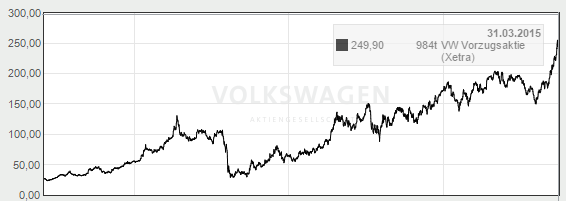
\includegraphics[width=0.7\textwidth]{images/finanzen2015}
\caption{Fünfjahresübersicht des VW-Börsenwerts \cite{aktienfotos}}
\label{fig:vwaktie1}
\end{figure}\FloatBarrier
\noindent
Wie in Abbildung \ref{fig:vwaktie1} zu sehen ist, ist der VW-Börsenwert in den letzten fünf Jahren stetig gestiegen, und wurde durch den Abgasskandal 2015 massiv erschüttert.
Der Stand vom 21. September 2015 der VW Börsenwert (Xetra) war nur mehr bei 60,89 Mrd. Euro.
\begin{figure}[!h]
\centering
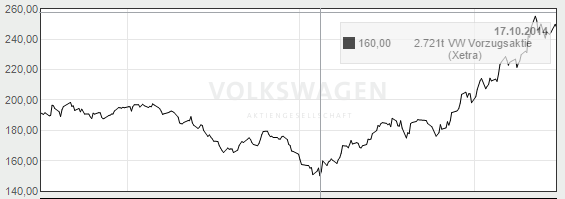
\includegraphics[width=0.6\textwidth]{images/finanzen20151}
\caption{Jahresübersicht der VW-Aktie 2015 \cite{aktienfotos}}
\label{fig:vwaktie3}
\end{figure}\FloatBarrier
\noindent
Mit Aufkommen des Skandals fiel die Aktie stetig, bis Mitte November ein leichter Gegentrend Einzug hielt.
\newpage
\textbf{Aktionärsstruktur}\\
Mit 31.12.2014 waren insgesamt 180.641.478 Vorzugsaktien und 295.089.818 Stammaktien ausstehend.\\
Im Juni 2014 hat die Volkswagen Aktiengesellschaft 10.471.204 neue Vorzugsaktien ausgegeben. Zusätzlich wurden im 1. Halbjahr 2014 22.103 Vorzugsaktien aus der Wandlung von Pflichtwandelanleihen geschaffen.
\cite{aktionaersstruktur} \\ \\
\textit{Übersicht über die Stimmrechtsverteilung} \\
50,73\% Porsche Automobil Holding SE, Stuttgart\\
20,00\% Land Niedersachsen, Hannover\\
17,00\% Qatar Holding LLC\\
12,30\% Andere\\
10\%, Louise Piech Privatstiftung\\
10\%, Louise Daxer-Piech\\
10\%, Ernst Piech Privatstiftung\\
10\%, Hans Michael Piech\\
10\%, Ferdinand Piech\\
12,5\%, Fam. Gerhard Porsche\\
12,5\%, Fam. Hans-Peter Porsche\\
12,5\%, Fam. Wolfgang Porsche\\
12,5\%, Fam. Ferdinand Alexander Porsche\\
\newpage

Die wichtigsten Zahlen hier noch einmal zusammengefasst: \cite{yahoofinanzenvw}
\begin{table}
\begin{tabular}{|p{0.75\textwidth}|p{0.25\textwidth}|}
\hline

\textbf{Geschäftsjahr 2015}  & = Kalenderjahr \\  \hline
\textbf{Rentabilität}  & \\  \hline
Gewinnspanne VW &   5,89\%  \\ \hline
Gewinnspanne Toyota & 9\% \\ \hline
Gewinnspanne GM & 3.8\% \\ \hline
 \textbf{Managementeffektivität}  & \\  \hline
Kapitalrentabilität  & 2,21\%  \\  
Eigenkapitalrendite  &   12,28\%  \\  \hline
 \textbf{GuV}  & \\  \hline

 Umsatz &   202,46Mrd. \\  
 Umsatz pro Aktie &  408,12  \\  
 
Vierteljährliches Umsatzwachstum &   6,60\% \\  
 Bruttoergebnis vom Umsatz &34,39Mrd.    \\  
EBITDA  &  20,50Mrd.  \\  
 Auf Stammaktien entfallender Jahresüberschuss  &  10,98Mrd.  \\  \hline
  \textbf{Bilanz}  & \\  \hline


Cash (gesamt) : &  	28,30Mrd.  \\  

Gesamt-Cash pro Aktie : & 59,50   \\  
Schulden (gesamt) : &   108,65Mrd. \\  
 Schulden/Equity (gesamt) :&  	120,47  \\  \hline
   \textbf{Cash Flow-Aufstellung}  & \\  \hline

Cash Flow aus betrieblichen Tätigkeiten  &  10,78Mrd.  \\  
Levered Cash Flow (wie viel Geld für Aktionäre übrig bleibt) & 8,45Mrd.  \\  \hline

\end{tabular}
\end{table}\FloatBarrier
\subsubsection{Übernahme von Porsche}

Im Oktober 2008 ist die Stammaktie von Volkswagen um 12 Milliarden gestiegen. Der Grund hierfür war, dass Porsche über drei Jahre hinweg einen Anteil an Volkswagen erworben hatte. \\
Die Chronik lässt sich wie folgt darstellen:\\\\
\textbf{2005}\\
Im Jahr 2005 begann die Firma Porsche AG Stammaktien der Firma VW zu kaufen. Bis Ende 2005 erwarben sie mit den liquiden Mitteln insgesamt 18\% der Stammaktien für etwa 3.5 Milliarden Euro. Porsche AG wollte in Volkswagen investieren, da sie selbst Angst vor einer Übernahme hatten und den Großkonzern zuerst kontrollieren wollte. Die beiden Firmen teilten sich damals bereits einige Produktionsstrukturen und waren allgemein sehr ähnlich. \\\\
\textbf{2006}\\
2006 steigerte Porsche den Anteil an VW auf 30\%.\\\\\\
\textbf{2007}\\
Die Porsche Holding SE, Stuttgart wird gegründet, in welche die Porsche AG  eingegliedert wird.\\ Die EU ändert ein Volkswagen internes Firmengesetz: Davor konnten Aktionäre nie mehr als 20\% Stimmrechte innehaben, ganz egal wie groß ihr Anteil ist. Da dies gegen EU-Regeln verstößt, wird dieses Gesetz abgeschafft.\\\\
\textbf{2008}\\
Porsche hat nun 35.14\% von Volkswagen inne, muss dafür jedoch einen Kredit von 6 Milliarden aufnehmen. \\
Dieser Kauf hat den Preis sehr hoch getrieben, weit über einen Wert, welcher wirtschaftlich sinnvoll war. Durch Spekulation wurden nun Aktien von sowohl Porsche, als auch VW gekauft und verkauft. Am 26 Oktober gab Porsche an, dass es nun 43\% von VW besitzt und die Möglichkeit hätte noch mehr zu kaufen, ein Interesse bestand, bis zu 75\% zu erwerben. \\
Daraufhin stieg der Preis der VW Aktien auf über 1000 Euro, und Volkswagen war für diese Zeit die Firma, welche weltweit am Meisten wert war. Der Kauf von Volkswagen schlägt fehl und die Verantwortlichen, Wendelin Wiedeking und Holger Härter werden entlassen.
\\\\
\textbf{2009}\\
Im Jänner hat Porsche nun 52\% der Volkswagen Group AG Aktien inne und Schulden in Höhe von 10 Milliarden Euro.
Aufgrund der Schulden hat die Familien Porsche Abschied davon genommen, ihren Anteil an VW auf 75 Prozent aufzustocken um den Konzern kontrollieren zu können und eine Not-Fusion mit Volkswagen entsteht. \\
Am 13. August wird ein Vertrag aufgesetzt, welcher den Vorstand von Volkswagen in den Aufsichtsrat der Porsche Holding SE erhebt. Des weiteren werden 49.9\% (um 3.9 Milliarden Euro) von der Porsche AG an Volkswagen verkauft. 10 \% der Porsche Holding SE gehen an Qatar Holding LLC. \\\\
\textbf{2011}\\
Eine Verschmelzung der Volkswagen Group und der Porsche Holding SE ist geplant, jedoch ist dies erst möglich, sobald alle Klagen gegen Porsche Holding SE beendet sind. Die in den Jahren zuvor (insbesondere Oktober 2008) hatten Klagen zur Folge. Die Porsche Holding SE wird der Marktmanipulation und der Absprache bezichtigt.\\\\
\textbf{2012}\\
Wegen den noch immer hohen Schulden verkauft die Porsche Holding SE die restlichen Anteile an die Porsche AG and Volkswagen um 4.5 Milliarden Euro.
\cite{squeezy}

\newpage
\subsection{Produktspektrum}
Im Mittelpunkt der Produktion steht das Automobil und wird von einer Anzahl an vielseitigen Dienstleistungen rund um das Thema Fahren verstärkt. Im finanziellen Sektor sind Dienstleistungen bereits auf eine eigene Gesellschaft "Volkswagen Financial Services" ausgelagert.
Das Produktspektrum der Volkswagen AG beinhaltet alle Kraftfahrzeuge vom Stadtfahrzeug, über Motorrad bis zum Großtransporter.
So unterteilt sich der Konzern in die folgenden Marken und Tochtergesellschafen:\\
\begin{figure}[!h]
\centering
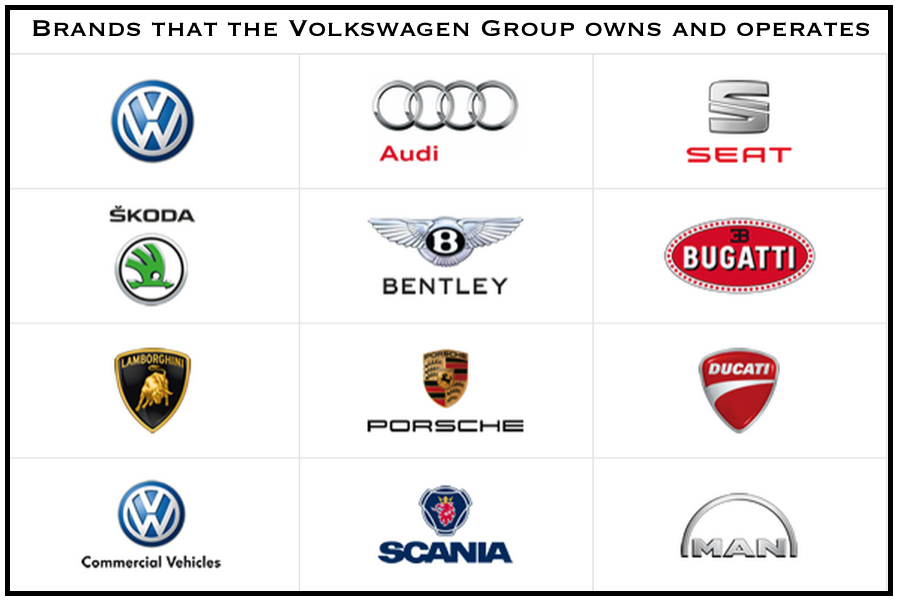
\includegraphics[width=0.9\textwidth]{images/Volkswagen-Group-Brands}
\caption{Marken und Tochtergesellschaften der Volkswagen AG. \cite{marken}}
\end{figure}\FloatBarrier
\noindent
\textbf{Volkswagen}\\
Das Segment von Volkswagen ist überwiegend auf den Endverbaucher abgestimmt. Das Spektrum reicht vom kleinen Stadtauto bis zum SUV. Einige bekannte Modelle darunter sind unter anderem Polo, Golf und Passat, Beetle, Sharan, Toureg, Tiguan.
Ebenso werden elektrisch betriebene Autos bzw. Fahrzeuge mit alternativem Antrieb angeboten.\\
\\
\textbf{Volkswagen Commercial Vehicles}\\
Die zweite eigene Untermarke des Konzerns konzentriert sich auf Transport und Nutzfahrzeuge. Die Modellpalette umfasst mitunter Vans, Hecklader und unterschiedliche Versionen von Transportern. Volkswagen Commercial Vehicles orientiert sich primär an den Bedürfnissen von Kunden, die aufgrund ihrer Tätigkeiten Kraft und Stauraum benötigen.
\newpage
\textbf{Audi}\\
Die Audi AG, welche symbolisch für den 1932 stattgefundenen Zusammenschluss von
Audi, DKW, Horch und Wanderer steht, produziert heute in den gängigen Klassen A, S, T, Q und weitere Kleinserien in der typischen Buchstabenbenennung. Mit der 'tron'-Technologie steht der Audi A3 Sportback auch in einer Hybrid-Version mit Benzin/Strom und Benzin/Erdgas zur Verfügung.
Seit mittlerweile 100 Jahren Produktion sind die Klassen in ihrer achten Generation angelangt, und bietet seinen Fahrern eine weitgestreute Modellpalette von Kleinwagen, über Sportwagen und SUV, bis zur Oberklasse. Die Audi AG bietet, sowie die zwei folgenden VW-Töchter Skoda und Seat für Unternehmen Business-Pakete an, in etwa Leasing für Firmenfahrzeuge.\\
\\
\textbf{Skoda}\\
Die Modelle der Marke Skoda sind eher in der Mittelklasse orientiert, bieten dem Fahrer allerdings zu günstigeren Preisen als manche andere Konzerntöchter, eine Vielzahl von aktuellen Features und neuen Technologien zum Thema Fahrkomfort und Sicherheit. Die gängigsten Modelle sind Fabia und Octavia.\\
\\
\textbf{Seat}\\
Der spanische Autohersteller Seat ist im Kleinwagen- und Mittelklassebereich angesiedelt. Der Konzern wurde 1950 ins Leben gerufen mit Unterstützung von Fiat, daher waren die ersten Modelle fast ausschließlich Lizenzbauten der Marke. Bereits drei Jahre danach wurde das erste werkseigene Serienmodell produziert und 1965 begann der Export in andere Länder.
Die gängigsten Serien der Marke sind heute unter anderen Ibiza, Leon und Alhambra, welche hauptsächlich in der Mittelklasse angesiedelt sind.\\
\\ 
\textbf{Porsche}\\
Der Premiumhersteller Porsche, welcher ursprünglich plante Volkswagen zu übernehmen, ging auf Grund von großen Schulden eine Zwangsallianz mit Europas größtem Autokonzern ein und wurde so schlussendlich doch ein Teil der Volkswagen Group.
Heute liegt er mit 18,4\% Gewinnmarge pro verkauften Modell trotzdem vor dem japanischen Massenhersteller Toyota, der aktuell die Spitze an verkauften Modellen pro Jahr führt.\\
Der Hersteller entwickelt ausschließlich Sportwagen, Oberklassenmodelle und SUV's.
Die gängisten Serien des Herstellers sind Cayenne, Boxster und 911, von denen 911 mit Carrera die größte Unterserie besitzt.\\
\\
\textbf{Lamborghini}\\
Der Luxushersteller produziert hauptsächlich Sportwagen und Coupes. Neben den Serienmodellen wurden auch eine
Vielzahl von Einzelmodellen entworfen, die in Design und Ergonomität überzeugen, was sich auch im Preis widerspiegelt.
\newpage
\textbf{Bentley}\\
Der Hoflieferant für die britische Königsfamilie, der ursprünglich lediglich als Schwestermarke der Firma Rolls-Royce bekannt war, ist seit 1919 ebenfalls für seine Modelle in der Ober- und Sportklasse bekannt.\\
\\
\textbf{Bugatti}\\
Die Luxusmarke Bugatti versucht mit zwei Serien, Veyron 16.4 und 16C Galibier, die Kraft von meist 12-zylindrigen Motoren in ein dennoch komfortables Reisefahrzeug zu integrieren. Die Preise der Modelle gehen in die Millionen.\\
\\
\textbf{Ducati}\\
Über den Tochterkonzern Audi kam die Motorradmarke Ducati zur Volkswagen Group. Die Produktpalette erstreckt sich bis zur schweren Rennmaschine, mit denen sich die Marke im Motorsport einen großen Namen gemacht hat.\\
\\
\textbf{Scania}\\
Das Sortiment des schwedischen Herstellers bietet Trucks für den simplen Transport bis hin zur Sonderfertigung von Einsatzfahrzeugen. Die Modelle des Herstellers umfassen ausschließlich Fahrzeuge für den Personen und Gütertransport. Stadt- und Reisebusse für Kurz- und Langstrecken sind ebenfalls mit inbegriffen.\\
Das Unternehmen arbeitet bereits länger eng mit der Volkswagen Group-eigenen LKW-Tochter MAN zusammen und wurde mit eben dieser zusammengeschlossen. Im Zuge der jahrelangen Verhandlungen wurde dieser Schritt erst spät gesetzt.\\
\\
\textbf{MAN}\\
MAN ist eine Tochter der Volkswagen Group, die LKWs produziert und ist somit der zweite Hersteller für Transport- und Reisefahrzeuge innerhalb der eigenen Firma. Das Angebot umfasst Transporter für Güter, Sattelschlepper, Reise und Stadtbusse.\\
\\
\textbf{Volkswagen Financial Services}\\
Die Dienstleistungen der Volkswagen Financial Services beschäftigen sich hauptsächlich mit der Finanzierung, dem Leasing und der Versicherung von Fahrzeugen eines Volkswagen-Kunden. Zusätzlich kommen noch Dienstleistungen wie Mobilitätsgarantie und direktes Banking hinzu. \cite{vw-produkte} \cite{audiRinge} \cite{audiNeuwagen} \cite{vwPorscheUebernahme}

\newpage
\subsection{Standorte}
Der Konzern betreibt über 118 Fertigungsstätten in denen rund 600.000 Personen beschäftigt sind.
Der Kern des Unternehmens sitzt in Deutschland, wobei Niedersachsen mit einem minimalen Überschuss die Sperrminorität und somit ein Vetorecht auf alle wichtigen Entscheidungen besitzt.
Der überwiegende Teil der Produktionsstätten ist nach Afrika und Asien ausgelagert, der Rest wird zum Teil in Amerika und Europa produziert.\\
Die folgenden Ländern gibt die Volkswagen Group an zu produzieren: \cite{produktionsstandorte}
\begin{table}[h]
	\begin{tabular}{|l|l|l|l|l|}
		\hline
		Argentinien          & Bosnien und Herzegowina & Brasilien & China    & \textbf{Deutschland}          \\ \hline
		Indien               & Mexiko                  & Polen     & Portugal & Russische Föderation \\ \hline
		Slowakische Republik & Spanien                 & Südafrika & USA      &                      \\ \hline
	\end{tabular}
\end{table}
\\

\subsection{Unternehmensstruktur}
"Die Volkswagen AG stellt die Muttergesellschaft des eigentlichen Volkswagen Konzerns da und entwickelt insbesondere Pkw und Nutzfahrzeuge für den Vertrieb, sowie Fahrzeuge und deren Komponenten für den Konzern. Der Vorstand der Volkswagen AG leitet das Unternehmen in eigener Verantwortung. \cite{struktur}

\subsubsection{Vorstand und Konzernleitung}
Das Gremium Konzernleitung trägt dafür Sorge, dass die Konzerninteressen bei Entscheidungen der Marken und Gesellschaften des Konzerns beachtet werden. Es besteht aus den Mitgliedern des Vorstands und ausgewählten Top-Managern mit Konzernsteuerungsfunktionen.\cite{struktur}
\newpage
\subsubsection{Vorsitzende des Vorstands der Volkswagen AG}
Obwohl das Unternehmen immer mehr Internationalität anstrebt und besonders in Amerika einen immer besseren Eindruck vermitteln möchte, kommt ein sehr großer Teil des neun Mann großen Vorstands aus Deutschland. Das liegt unter anderem daran das Volkswagen auch heute noch einen sehr großen Teil seiner Geschäfte in deutschsprachigen, beziehungsweise europäischen Ländern abwickelt.\cite{vorstand} \\ \\
\textbf{Vorstandsvorsitzender}
\begin{figure}[!h]
	\centering
	\begin{minipage}[h]{0.20\textwidth}
		\centering
		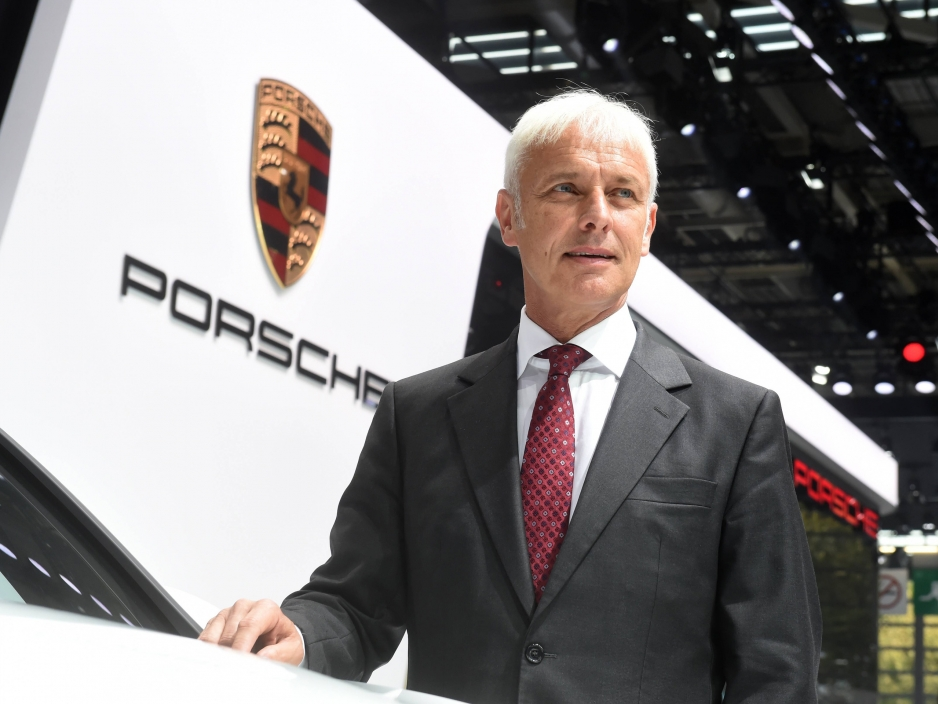
\includegraphics[width=1.0\textwidth]{images/MathiasMueller.jpg}
		\label{fig:vorstandvw0}
	\end{minipage}
		\begin{minipage}[h]{0.10\textwidth}
		\hspace{1cm} 
	\end{minipage}
	\begin{minipage}[h]{0.65\textwidth}
		Matthias Müller ist Vorstandsvorsitzender der Volkswagen AG, Vorstandsmitglied der Porsche-Holding sowie Aufsichtsratsvorsitzender bei Audi. Nach dem Rücktritt von Martin Winterkorn im September 2015 im Zuge des Abgasskandals wurde Matthias Müller am 25. September 2015 neuer Vorstandsvorsitzender der Volkswagen AG. Wenige Wochen später wurde er auch zum Aufsichtsratsvorsitzenden der Audi AG gewählt.(Bild: \cite{mmpic} )

	\end{minipage}
\end{figure}\FloatBarrier\noindent

\textbf{Mitglieder des Vorstands}
\begin{figure}[!h]
	\centering
	\begin{minipage}[h]{0.65\textwidth}
		Dr. rer. pol. h. c. Francisco Javier Garcia Sanz ist seit dem 1. Juli 2001 Vorstandsmitglied der Volkswagen AG. Sein Geschäftsbereich ist 'Beschaffung'. Zusätzlich ist er schon seit dem 30. November 1996 Vorsitzender der Marke Volkswagen PKW bei der er ebenfalls dem Geschäftsbereich 'Beschaffung' zugeteilt ist. Seit Juni 2007 ist Francisco Javier Garcia Sanz Vorsitzender des Verwaltungsrats der SEAT, S.A. (Barcelona). (Bild: \cite{fspic} )
	\end{minipage}
		\begin{minipage}[h]{0.10\textwidth}
		\hspace{1cm}
	\end{minipage}
	\begin{minipage}[h]{0.20\textwidth}
		\centering
		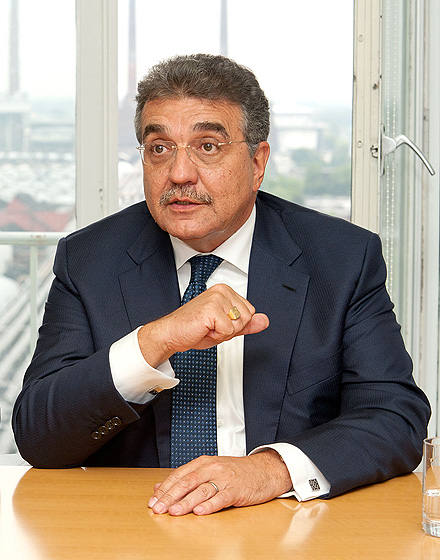
\includegraphics[width=1.0\textwidth]{images/FranciscoSanz.jpg}
		\label{fig:vorstandvw1}
	\end{minipage}
\end{figure}

\begin{figure}[!h]
	\centering
	\begin{minipage}[h]{0.20\textwidth}
		\centering
		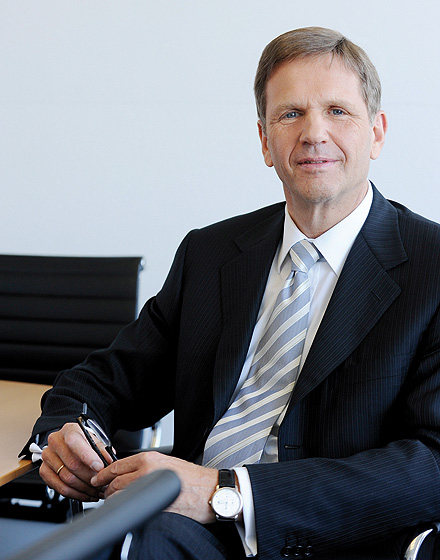
\includegraphics[width=1.0\textwidth]{images/JochemHeizmann.jpg}
		\label{fig:vorstandvw2}
	\end{minipage}
	\begin{minipage}[h]{0.10\textwidth}
		\hspace{1cm} 
	\end{minipage}
	\begin{minipage}[h]{0.65\textwidth}
		Der Aufsichtsrat der Volkswagen AG beruf Prof. Dr. rer. pol. Dr.-Ing. E. h. Jochem Heizmann am 1. September 2012 zu einem Mitglied des Vorstands für den Geschäftsbereich 'China'. Er nimmt diese Position zusätzlich zu seiner Funktion als President und CEO der Volkswagen Group China wahr. Vom 1. Oktober 2010 bis zum 31. August 2012 verantwortete Prof. Dr. Heizmann weiters als Mitglied des Vorstands der Volkswagen AG den Geschäftsbereich 'Konzern Nutzfahrzeuge'. (Bild: \cite{jhpic} )
	\end{minipage}
\end{figure}

\begin{figure}[!h]
	\centering
	\begin{minipage}[h]{0.65\textwidth}
		Von 2004 bis 2008 war Christian Klingler Mitglied der Geschäftsführung der Porsche Holding Österreich.
		Im August 2008 wurde Christian Klingler als Generalbevollmächtigter der Volkswagen AG in den Vorstand der Marke Volkswagen berufen und war verantwortlich für die Bereiche Vertrieb und Marketing sowie After Sales. Seit dem 1. Januar 2010 ist Klingler zusätzlich Mitglied des Vorstands der Volkswagen AG und zuständig für den Geschäftsbereich 'Vertrieb und Marketing'  (Bild: \cite{ckpic} )
	\end{minipage}
	\begin{minipage}[h]{0.10\textwidth}
		\hspace{1cm} 
	\end{minipage}
	\begin{minipage}[h]{0.20\textwidth}
		\centering
		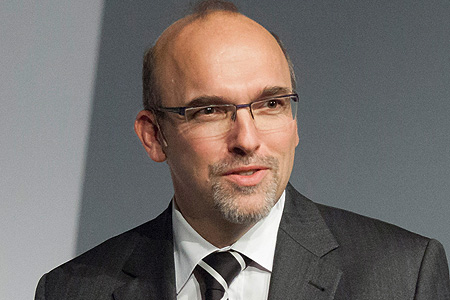
\includegraphics[width=1.0\textwidth]{images/ChristianKlingler.jpg}
		\label{fig:vorstandvw3}
	\end{minipage}
\end{figure}

\begin{figure}[!h]
	\centering
	\begin{minipage}[h]{0.65\textwidth}
		Seit Juli 2002 ist Dr. Horst Neumann Mitglied des Vorstands der AUDI AG und damit verantwortlich für den Geschäftsbereich Personal- und Sozialwesen. Zum 1. Dezember 2005 bestellte ihn der Aufsichtsrat der Volkswagen AG zum Mitglied des Vorstands der Volkswagen AG  der Marke Volkswagen für den Bereich "Personal, Arbeitsdirektor". Seit Januar 2007 ist er verantwortlich für Personal und Organisation. (Bild: \cite{hmpic} )
	\end{minipage}
	\begin{minipage}[h]{0.10\textwidth}
		\hspace{1cm} 
	\end{minipage}
	\begin{minipage}[h]{0.20\textwidth}
		\centering
		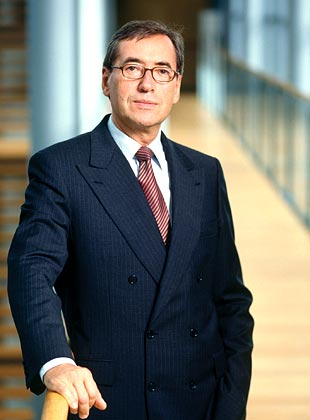
\includegraphics[width=1.0\textwidth]{images/HorstNeumann.jpg}
		\label{fig:vorstandvw5}
	\end{minipage}
\end{figure}

\begin{figure}[!h]
	\centering
	\begin{minipage}[h]{0.20\textwidth}
		\centering
		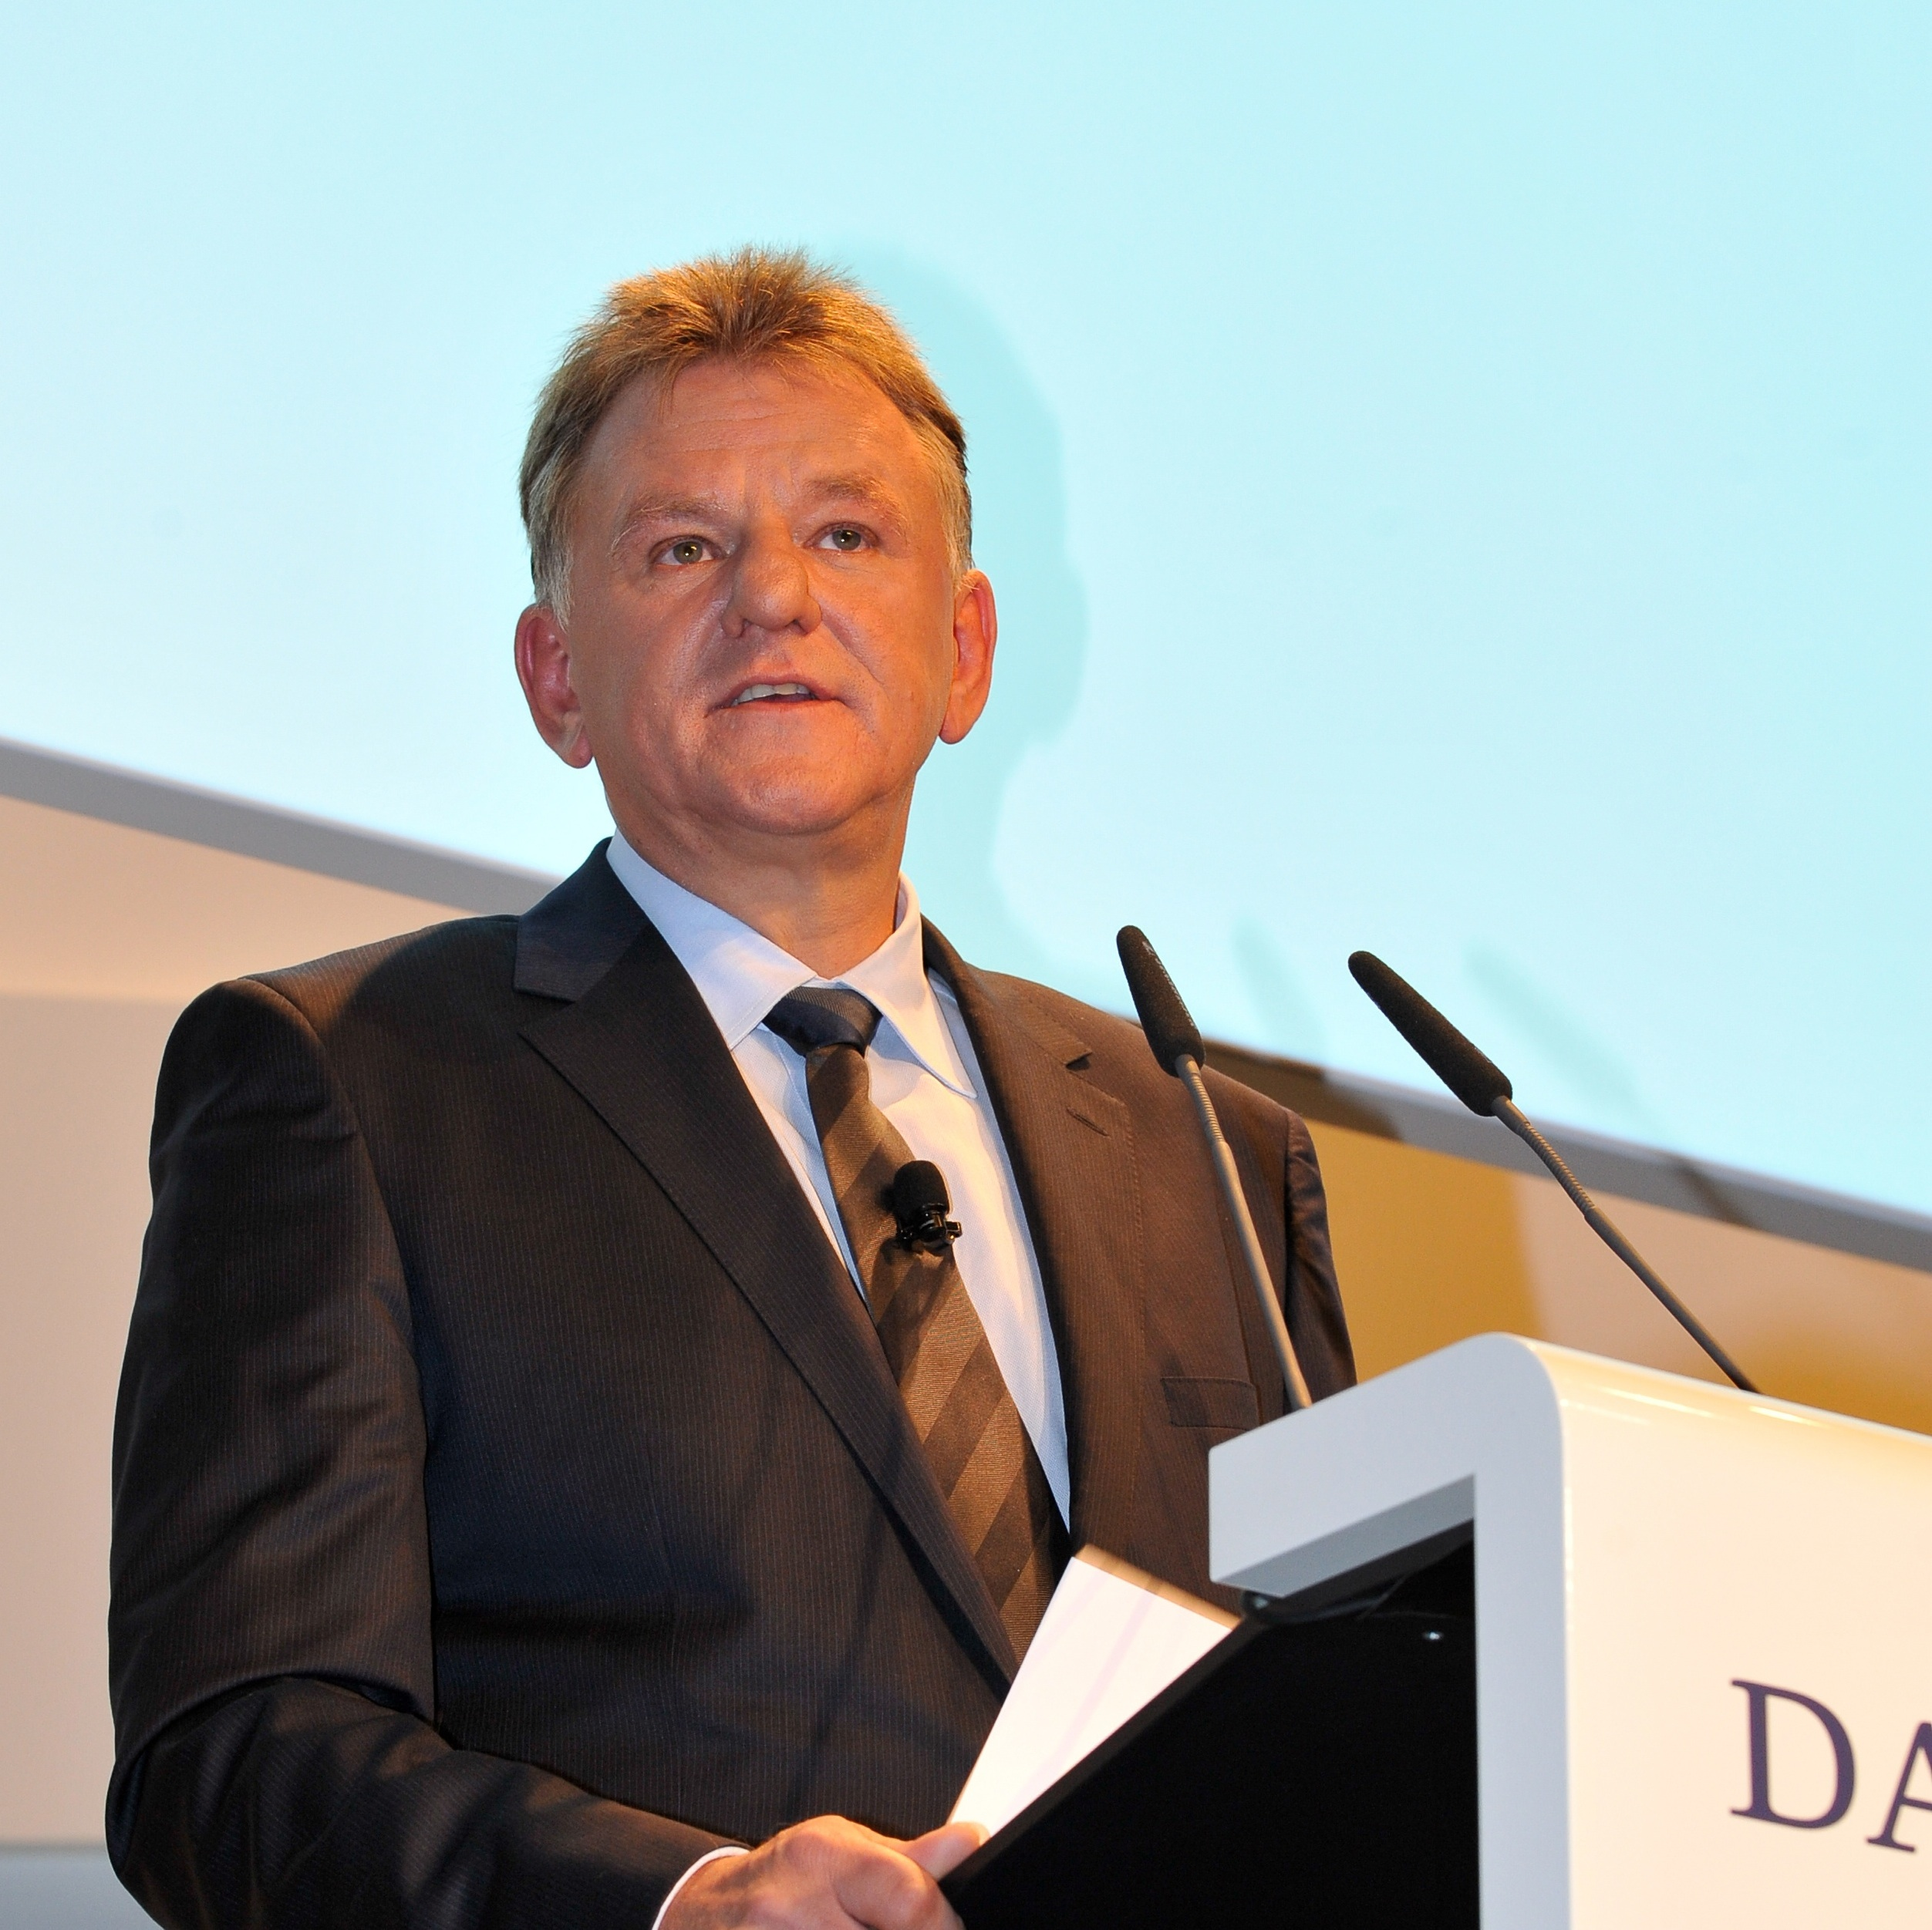
\includegraphics[width=1.0\textwidth]{images/AndreasRenschler.jpg}
		\label{fig:vorstandvw6}
	\end{minipage}
	\begin{minipage}[h]{0.10\textwidth}
		\hspace{1cm} 
	\end{minipage}
	\begin{minipage}[h]{0.65\textwidth}
		Früher wurde Andreas Renschler bei Mitsubishi Motors in Japan und der Daimler AG im Bereich Daimler Trucks eingesetzt. Seit 1. Februar 2015 ist er Mitglied des Vorstands der Volkswagen AG im Geschäftsbereich 'Nutzfahrzeuge'. (Bild: \cite{arpic} )
	\end{minipage}
\end{figure}

\begin{figure}[!h]
	\centering
	\begin{minipage}[h]{0.65\textwidth}
		"Der Aufsichtsrat der Volkswagen AG übertrug Dipl. Wirtsch.-Ing. Hans Dieter Pötsch mit Wirkung zum 5. September 2003 die Verantwortung für den Geschäftsbereich ‘Finanzen und Controlling‘ auf Konzernebene im Vorstand. Bereits zum 1. Januar 2003 hatte der Aufsichtsrat Pötsch zum ordentlichen Mitglied des Vorstands, zunächst ohne Geschäftsbereich, berufen. Seit dem 25. November 2009 ist Hans Dieter Pötsch zusätzlich zu seinen bisherigen Funktionen im Vorstand der Porsche Automobil Holding SE, Stuttgart, vertreten. Er nimmt dort ebenfalls die Position des Finanzvorstands ein."\cite{poetschbio}  (Bild: \cite{dppic} )
	\end{minipage}
	\begin{minipage}[h]{0.10\textwidth}
		\hspace{1cm} 
	\end{minipage}
	\begin{minipage}[h]{0.20\textwidth}
		\centering
		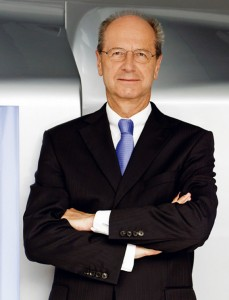
\includegraphics[width=1.0\textwidth]{images/HansPoetsch.jpg}
		\label{fig:vorstandvw7}
	\end{minipage}
\end{figure}

\begin{figure}[!h]
	\centering
	\begin{minipage}[h]{0.20\textwidth}
		\centering
		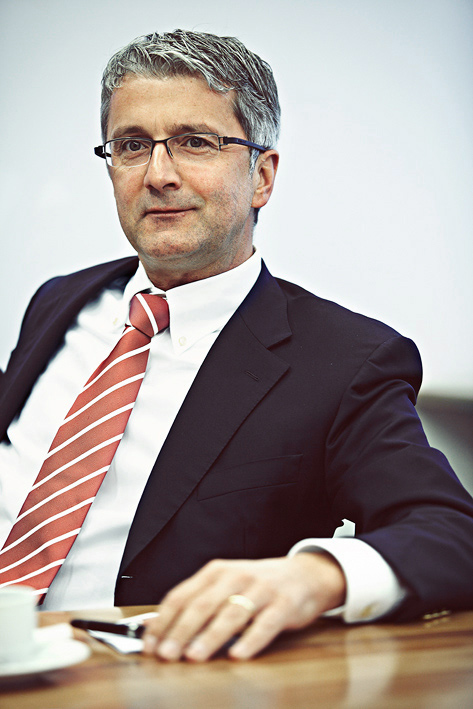
\includegraphics[width=1.0\textwidth]{images/RupertStadler.jpg}
		\label{fig:vorstandvw8}
	\end{minipage}
	\begin{minipage}[h]{0.10\textwidth}
		\hspace{1cm} 
	\end{minipage}
	\begin{minipage}[h]{0.65\textwidth}
		Prof. Rupert Stadler ist seit dem 1. Januar 2003 Mitglied des Vorstandes der Audi AG. Am 1. April 2003 übernahm er die Verantwortung für den Geschäftsbereich Finanz und Organisation. Seit 1. Januar 2007 ist Rupert Stadler Vorsitzender des Vorstands der Audi AG. Den Geschäftsbereich Finanz und Organisation führte er in Personalunion bis 31. August 2007 weiter. Rupert Stadler wurde in seiner Funktion als Vorsitzender des Vorstands der Audi AG zum 1. Januar 2010 in den Vorstand der Volkswagen-Aktiengesellschaft berufen. (Bild: \cite{rspic} )
	\end{minipage}
\end{figure}
\cite{vorstand}

\subsubsection{Marken und Hierarchie}
Jede Marke des Volkswagen Konzerns wird von einem Markenvorstand geleitet. Dabei sind die vom Vorstand der Volkswagen AG beziehungsweise von der Konzernleitung festgelegten Konzernziele und -vorgaben und die jeweiligen rechtlichen Rahmenbedingungen zu beachten. Angelegenheiten von konzernweiter Bedeutung werden der Konzernleitung vorgelegt.
Die einzelnen Gesellschaften des Volkswagen-Konzerns werden jeweils unter Verantwortung einer eigenen Geschäftsleitung geführt. Dabei berücksichtigen die jeweiligen Geschäftsleitungen neben den Interessen der Gesellschaft auch Konzern- und Markeninteressen.\cite{structure1}
Die Hierarchie sieht dabei wie folgt aus:

\begin{table}[h]
	\begin{tabular}{|c|c|c|c|c|c|c|c|c|}
		\hline
		\multicolumn{7}{|c|}{Volkswagen AG}                                                                                                                                                     \\ \hline
		\multicolumn{3}{|c|}{Volkswagen} & \multicolumn{2}{c|}{Audi} & \multicolumn{1}{c|}{\begin{tabular}[c]{@{}c@{}}Volkswagen\\ Nutzfahrzeuge\end{tabular}} & \multicolumn{1}{c|}{Weitere} \\ \hline
		Skoda    & Bugatti   & Bentley   & Seat     & Lamborghini    & MAN/Scania                                      & Porsche       \\ \hline
	\end{tabular}
\end{table}

Die Volkswagen AG ist grundsätzlich schon immer durch die starke Eigenständigkeit der verschiedenen Marken geprägt. Die Marken sind beispielsweise für Produktdesign, Vertrieb, Marketing und vieles mehr weitgehend eigenständig. Sogar die Produktionsstandorte und Werke sind meistens einer einzelnen Marke zugeteilt und werden von dieser organisiert.
\cite{domavw}
\newpage
\subsection{Logistik}
\begin{figure}[!h]
	\centering
	
\includegraphics[width=0.7\textwidth]{images/logologistics.jpg}
	\caption{Logo der Volkswagen Logistics GmbH \& Co. OHG}
	\label{fig:vwlogisticspic}
	\cite{vwlogisticspic}
\end{figure}\FloatBarrier
Die Logistikprozesse der Volkswagen AG werden durch den Dienstleister Volkswagen Logistics GmbH \& Co. OHG gesteuert und verwaltet.
Volkswagen Logistics übernimmt hierbei nicht nur integrierte Logistik bei Volkswagen, sondern auch externe Aufträge für Dienstleister und Kunden.\cite{vwlogistics}

\subsubsection{Leitung und Sitz}
Volkswagen Logistics GmbH \& Co. OHG hat seinen Sitz in Wolfsburg und wird von Thomas Zernechel und Dinah J. Kamiske geleitet.
Das Unternehmen agiert mit seinen 600 Mitarbeitern international auf über 130 Märkten.\cite{vwlogistics}

\subsubsection{Zuständigkeit}
Volkswagen Logistics betreut dabei die gesamte Supply Chain, angefangen beim Lieferanten, über die Produktions- und Distributionsstufen, bis hin zur Auslieferung beim Kunden.\\
Volkswagen Logistics ist außerdem für die Lagerung, den Transport und die Verpackung von Produkten zuständig. Zusätzlich übernimmt Volkswagen Logistics auch die Entsorgungslogistik, die sowohl bei der normalen Produktion, als auch bei der Entwicklung von Prototypen eine sehr wichtige Rolle spielt.\cite{vwlogistics}

\subsubsection{Besonderheiten}
43 Milliarden Teile werden jährlich allein innerhalb des Volkswagen-Konzerns transportiert. Um dies zu ermöglichen, ist daher eine starke und flexibel agierende Logistik unverzichtbar.
Innovation und Ideen haben bei Volkswagen Logistics einen hohen Stellenwert. Volkswagen Logistics ist überzeugt, dass nur mithilfe modernster Technologien und Optimierungen ein Wettbewerbsvorteil erreicht werden kann.

Im Rahmen einer Fachtagung, des so genannten "Innovationstag Logistik", stellte Volkswagen 2013 einige ihrer Besonderheiten vor. Bemerkenswerte Technik mit denen Volkswagen arbeitet sind unter anderem lasergesteuerte, fahrerlose Transportsysteme zur automatisierten Materialbereitstellung, ergonomische Handschubwagen mit Elektroantrieb und besondere Roboter, die eigens für bestimmte Logistikprobleme entwickelt wurden.\cite{wolfsburg}
\subsection{Plattformstrategie}
Volkswagen verwendet schon seit sehr langer Zeit sogenannte modulare Baukastenstrategien, um die Kosten der Fahrzeugentwicklung zu senken. Das neueste, 2012 eingeführte, Mitglied der Baukastenfamilie ist der modulare Querbaukästen (kurz MQB). Er ist die Weiterentwicklung der Plattform- und Modulstrategie, die Volkswagen gegen Mitte der 90er Jahre entwickelt hat. Der MQB wird als Basis für Fahrzeuge, deren Motor quer zur Fahrtrichtung gebaut ist, verwendet. Der neue Audi A3, der neue Golf, der Seat Leon und der Seat Octavia basieren unter anderem auf diesem modularem Baukasten. Weiters gibt es noch viele andere modulare Baukästen, zum Beispiel der sehr ähnliche modulare Längsbaukasten (MLB).\cite{mqb}
\FloatBarrier
\begin{figure}[!h]
	\centering
	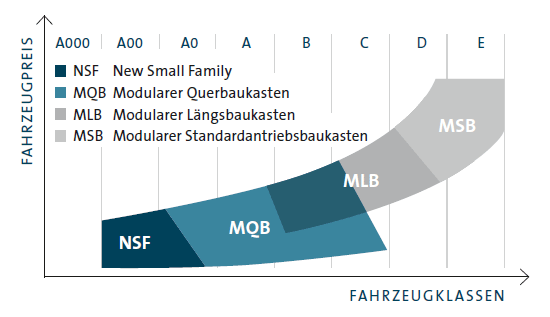
\includegraphics[width=0.7\textwidth]{images/MQB}
	\caption{Verschiedene Baukästen für verschiedene Klassen \cite{baukastengraph}}
\end{figure}\FloatBarrier\noindent

Hinter diesen modularen Baukästen steckt die Idee, dass Autos einander ähneln. Auch wenn Autos sich optisch oder auch funktional unterscheiden, bleiben viele Teile sehr ähnlich. Deshalb wurden sogenannte Plattform Strategien (von Volkswagen Baukastenstrategien genannt) entwickelt. Diese definieren Grundgerüste die zur Entwicklung verschiedenster Autos verwendet werden. \\ "Mit dem MQB ist eine hochflexible Fahrzeugarchitektur entstanden, bei der konzeptbestimmende Abmessungen wie Radstand, Spurbreite, Rädergröße und Sitzposition konzernweit abgestimmt sind und variabel zum Einsatz kommen. Andere Abmessungen, zum Beispiel der Abstand der Pedale zur vorderen Radmitte, sind immer gleich und gewährleisten eine einheitliche Systematik des Vorderwagens."\cite{mqb}
\FloatBarrier
\begin{figure}[!h]
	\centering
	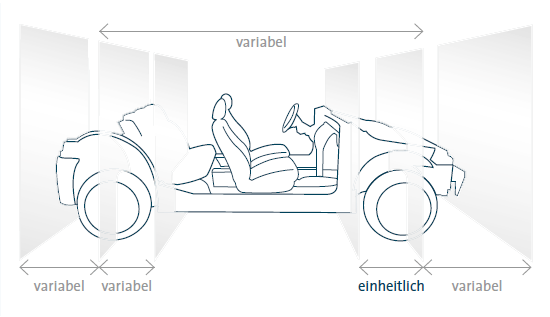
\includegraphics[width=0.7\textwidth]{images/MQB2}
	\caption{Grundarchitektur eines MQB-Fahrzeugs \cite{mqbdefault}}
\end{figure}\FloatBarrier
\newpage\newpage
\subsection{Markt}
Die Volkswagen Group, also alle Untermarken von VW gemeinsam, produziert global am meisten PKWs, jedoch führen Toyota sowie General Motors noch vor Volkswagen den globalen, totalen Verkauf an Fahrzeugen aller Klassen. \\
In 2013 wurden von Volkswagen etwa 9.3 Millionen Autos produziert. \\
Toyota kommt aus Japan und dominiert sowohl den japanischen als auch den amerikanischen Markt. GM kommt aus Amerika - daher dominieren sie hier traditionell den amerikanischen Markt.

\newpage
\textbf{Weltweit}\\
Wie in Abbildung \ref{fig:marktwelt} ersichtlich ist, führt Volkswagen den Marktanteil bei PKWs weltweit an. 

\begin{figure}[!h]
\centering
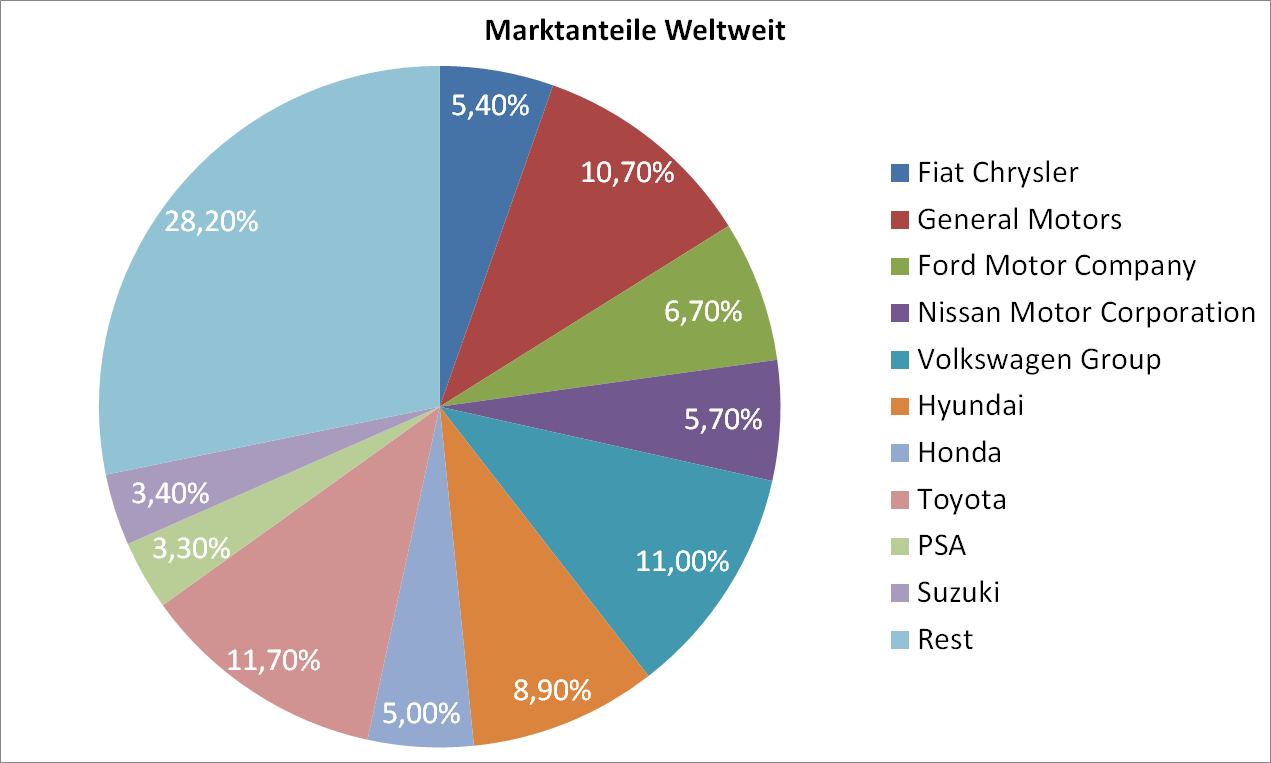
\includegraphics[width=1.0\textwidth]{images/maww}
\caption{Der Marktanteil Weltweit (PKWs)}
\label{fig:marktwelt}
\end{figure}\FloatBarrier
\noindent
\textbf{Europa}\\
Wie in Abbildung \ref{fig:markteuropa} ersichtlich ist, führt Volkswagen den Marktanteil in Europa bei weitem an. Die Tendenz ist steigend.
\begin{figure}[!h]
\centering
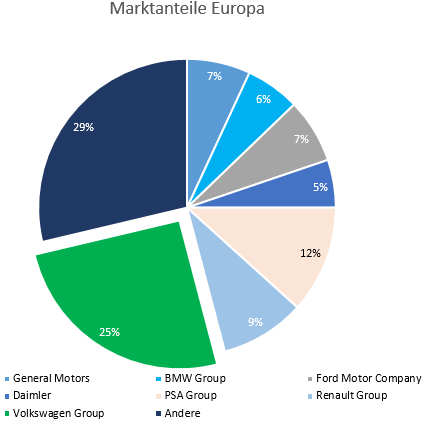
\includegraphics[width=0.7\textwidth]{images/maie}
\caption{Der Marktanteil in Europa (PKWs)}
\label{fig:markteuropa}
\end{figure}\FloatBarrier
\noindent
\textbf{Asien}\\
"Seit Beginn seiner Reform- und Öffnungspolitik vor über 30 Jahren ist China zu einem der wichtigsten Automobilmärkte der Welt aufgestiegen und bildet inzwischen den größten Absatzmarkt des Volkswagen Konzerns. Mit einem Anteil von 20,8 \% am Pkw-Markt und 3,27 Millionen verkauften Fahrzeugen im Geschäftsjahr 2013 ist der Volkswagen Konzern Marktführer in China."\cite{vwwebsitechina}\\
Volkswagen war einer der ersten Autohersteller die China nicht nur als Absatzmarkt sondern auch als Produktionsstandort betrachtet hat und daher stark mit der kommunistischen Führung in China kooperiert hatte. Dadurch konnte Volkswagen sich bis heute in Asien, insbesondere jedoch in China sehr gut positionieren: 
"Die kommunistische Führung in China lässt ausländische Investoren aus Schlüsselbranchen wie der Autoindustrie nur mit inländischen Partnern agieren - in Gemeinschaftsunternehmen (Joint Ventures). Damit soll verhindert werden, dass die ausländischen Marken den Markt alleine dominieren." \cite{vwamstrategiechina2}\\
Durch das dort ansässige Unternehmen Shanghai-Volkswagen Automotive Company (SVW) sowie des Unternehmens FAW-Volkswagen Automotive Company Ltd. (FAW-VW) konnten daher viele Produktionsstandorte in China aufgebaut werden.
Asien, insbesondere China, zeichnet sich durch eine stetig steigende Nachfrage aus. So wurden inzwischen etwa 17 Gesellschaften (Komponenten-, Finanz- und Vertriebsgesellschaften) in Asien gegründet. \\
Ende der 90er Jahre wurde auch in Asien verstärkt mit der Diversifikation der Produktpalette begonnen. Das  Produktportfolio in Asien umfasst heute alle Segmente vom Kleinwagen bis zum Luxussportwagen.
\\
Mit seinem umfangreichen Produktportfolio, neuesten Technologien sowie den Planungen zu Hybrid- und Elektrofahrzeugen ist der Volkswagen Konzern bestens gerüstet, um zukünftigen Herausforderungen – zum Beispiel anspruchsvollen Emissionsgrenzen oder Zulassungsbeschränkungen in Megacitys – zu begegnen und auch langfristig eine Schlüsselrolle auf dem Automobilmarkt in Asien innezuhaben. \\
In China herrscht des weiteren ein sehr ausgeprägtes Marken bewusstsein und die Volkswagen Group gilt dort als guter europäischer Fahrzeugbauer.  Eine Strategie von Volkswagen um in Asien noch besser positioniert zu sein, ist eher auf die individuellen Bedürfnisse der Asiaten (Chinesen sind zum Beispiel in der Regel kleiner und leichter) einzugehen. \cite{vwamstrategiechina}
\begin{figure}[!h]
\centering
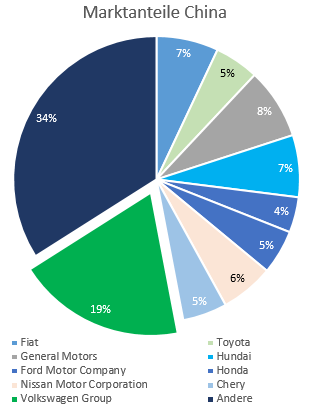
\includegraphics[width=0.45\textwidth]{images/mach}
\caption{Der Marktanteil in China (PKWs)}
\label{fig:marktchina}
\end{figure}\FloatBarrier
\noindent
\textbf{Japan} \\
Volkswagen konnte in Japan kaum Fuß fassen, unter anderem auch da Japan einige eigene Marken hervorgebracht hat.  Die Volkswagen Group kommt in Japan nur unter der Kategorie 'Andere' vor. Volkswagen selbst sieht jedoch das japanische Marktsegment als nicht erstrebenswert zu erklimmen, da es sehr schwierig ist die lokalen Anbieter dort zu vertreiben.
\\\\
\textbf{Nordamerika}\\
Volkswagen konnte sich in Amerika noch nicht durchsetzten. Derzeit hat Volkswagen nur 4\% des Marktanteiles (Verglichen mit 25\% in Europa) inne, wie man in Abbildung \ref{fig:marktnordamerika} sehen kann. Dies zu steigern ist ein Ziel der kommenden paar Jahre. Die Autos haben zwar als deutsche Qualitätsware einen guten Ruf, jedoch fehlt in Amerika auch die nötige Infrastruktur, also Händler und Werkstätten. \\ Des Weiteren werden in Amerika mehr SUVs und Pick-Ups gekauft, ein Segment in welchem Volkswagen nicht unbedingt stark vertreten ist.\\
Trotzdem konnte Volkswagen 2012 die besten Verkaufszahlen seit dem Käfer erwirtschaften und laut eigenen Angaben sollen ab 2018 mindestens 800.000 Autos pro Jahr verkauft werden. In den ersten fünf Monaten von 2014 jedoch ist der Verkauf wieder um 15\% gefallen, zu Gunsten von GM. Jedoch erwartet Volkswagen, dass mit der Einführung des neuen Golfes ihr Marktanteil steigen wird. Porsche und Audi verkaufen sich sehr gut in Nordamerika. \cite{vwamstrategiechina} \\
Mit nur circa 400.000 verkauften Neuwagen in 2013 - um 7\% weniger als im Vorjahr - ist es nicht klar, ob das Ziel bis 2018 in Amerika noch erreicht werden kann.\cite{ec1}\\
Amerika ist daher der - neben Japan - am schwierigsten zu erschließende Markt.
\begin{figure}[!h]
\centering
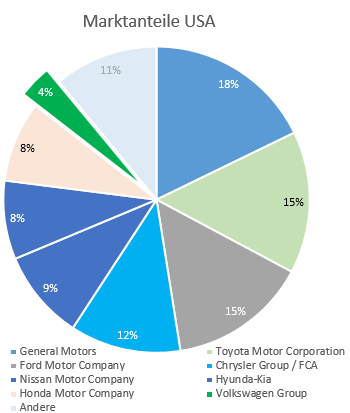
\includegraphics[width=0.7\textwidth]{images/maam}
\caption{Der Markt in den USA als Beispiel für Nordamerika (PKWs)}
\label{fig:marktnordamerika}
\end{figure}\FloatBarrier
\noindent
\\\\
\textbf{Südamerika}\\
In Südamerika ist Volkswagen relativ gut vertreten. Fiat führt zwar den Markt an, aber dicht gefolgt von Volkswagen. \\
Jedoch hatten sie dort eine Umsatzeinbusse in den letzten Jahren.







\subsection{Ziele und Zukunftsaspekte}
Laut der Volkswagen Website steht bis 2018 die Positionierung des Konzerns als weltweit führend sowohl ökonomisch und ökologisch an erster Stelle.\\ Das Toyota 2015 allerdings mit Einbußen im Heimatland Japan rechnet konnte es VW 2015 schaffen erstmals der größte Autohersteller der Welt zu werden - dieses Ziel hätte erst 2018 verwirklicht werden sollen.\\
Zur Erreichung und Instandhaltung der Konzernziele wurden vier offizielle Subziele (\cite{vwwebsitestrat}) definiert:
\begin{enumerate}
\item Steigerung der Kundenzufriedenheit und Qualität. Erreichung einer höheren Kundenzufriedenheit für nachhaltigen Erfolg.
\item Der Absatz soll von 9.259 Mio Fahrzeuge auf mehr als 10 Mio. Fahrzeuge gesteigert werden.  Vor allem auf die expandierenden Märkte in Asien sowie der noch schwach genützte Markt von Nordamerika soll ein stärkeres Augenmerk gelegt werden.
\begin{figure}[!h]
\centering
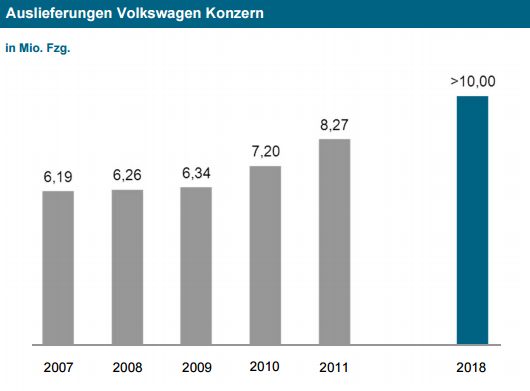
\includegraphics[width=0.4\textwidth]{images/strategie}
\caption{ Wachstumsstrategie \cite{vwamstrategie3}}
\end{figure}\FloatBarrier
\noindent
\item Die Umsatzrendite vor Steuern soll nachhaltig mindestens 8\% betragen, damit die finanzielle Stabilität und Handlungsfähigkeit des Konzerns auch in schwierigen Marktphasen sichergestellt ist. 
\item Volkswagen will sich auch als Arbeitgeber besser profilieren, um so höher qualifizierte Mitarbeiter gewinnen zu können.  \\\\
Des weiteren sind folgende Ziele immer wieder zu erkennen: \\
\item Volkswagen will auf dem amerikanischen Markt stärker präsent sein. Um genau dies zu schaffen, muss Volkswagen den Giganten Toyota vertreiben. \cite{ec1}
\item Volkswagen will in wachsenden Märkten vor allem mit dem neuen e-Golf und dem e-Up! Position beziehen. Elektro Fahrzeuge wurden Anfang 2000 noch kategorisch von der Firmenspitze abgelehnt. \cite{ec3} 
\item Es sollen umweltverträglichere und vor allem spritsparende Autos entwickelt und produziert werden, um so mit dem derzeitigem globalen Trend von Nachhaltigkeit mithalten zu können. Durch ein Baukastensystem sowie einen Leichtbau des Fahrzeuges sollen neue ökologische Maßstäbe gesetzt werden.
\item Natürlich soll die führende Position von Volkswagen in Europa beibehalten werden und finanzielle Rücklagen ausreichend gebildet werden.
\item Das Wettrennen gegen GM und Toyota soll weniger stark angegangen werden, so dass Volkswagen will zukünftig versuchen seine Gewinnspanne pro Auto zu steigern. Sie wollen mehr auf das Baukastensystem setzten. So sollen die Stückkosten um 20\% gesenkt werden und die Bauzeit pro Auto um 30 \% verkürzt werden. \cite{vwamstrategie}
\item Die Volkswagengroup besitzt mit der bereits einen überwiegenden Teil an Stimmrechten und Kapital der schwedischen Marke Scanias und plant eine Integration mit der eigenen LKW-Tochter MAN. Dieser Entschluss wird derzeit allerdings von Experten der International Strategy \& Investment London sehr kritisch betrachtet, da die Komplettübernahme des Herstellers der Volkswagen Group 8.6 Milliarden Euro wert ist. Ein betrag der in keinem Verhältnis zu den dafür errechneten Profiten von 1.8 Milliarden Euro in den nächsten Jahren steht. Die Volkswagen Group rechtfertigt diese Transaktion mit dem Aufheben von Barrieren die das Optimum aus der Zusammenarbeit von Scania und MAN herausholen soll.
Im laufenden Jahr 2015 sollen 40 bis 50 Prozent der geplanten Übernahme aus dem Cashflow finanziert werden. \cite{ScaniaMAN}
\end{enumerate}
\newpage
\section{Auswahl eines ERP Systemes}
\subsection{Itelligence AG}
\begin{figure}[!h]
\centering
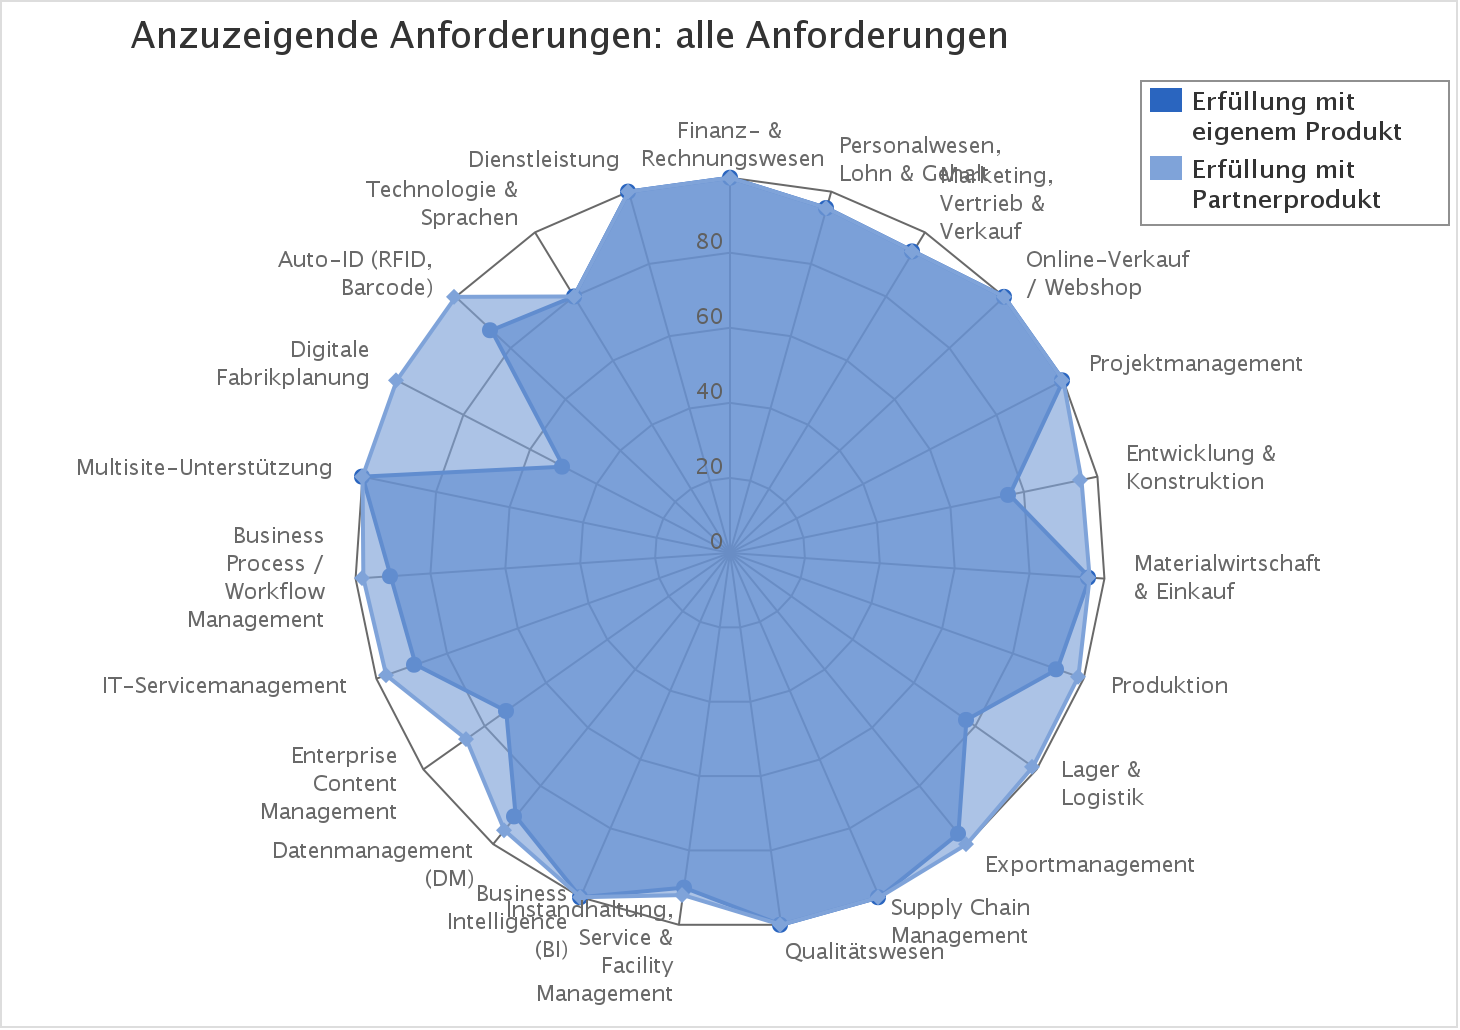
\includegraphics[width=0.7\textwidth]{images/TROVARIT_itelligence_AG}
\caption{Das Spinnennetz von Itelligence AG}

\end{figure}\FloatBarrier
\noindent


\begin{itemize}
\item itelligence ERP Branchenlösungen \\
		90\% Erfüllung mit eigenem Produkt\\
		97\% Erfüllung mit Partnerprodukt\\
		
		Nachteile: Man kann keinen Skill-Kataloge bezüglich der Mitarbeiter anlegen, außerdem kann im Bereich des Facility Managements keine Parkplätze und Reinigungen verwaltet werden.
Social Media Marketing wird auch nicht unterstützt.
Beim Vertrieb und Verkauf werden keine Touch Oberflächen unterstützen und die Tastenbelegung ist nicht frei konfigurierbar. Bei der Gestaltung wird keine 5D-Visualisierung unterstützt und bei der Planung können keine White- und Dashboards mit der Software verarbeitet werden. Außerdem ist dieses ERP System nicht Datenbankunabhängig.

		
		
\subsection{Microsoft Dynamics AX 2012}
\begin{figure}[!h]
\centering
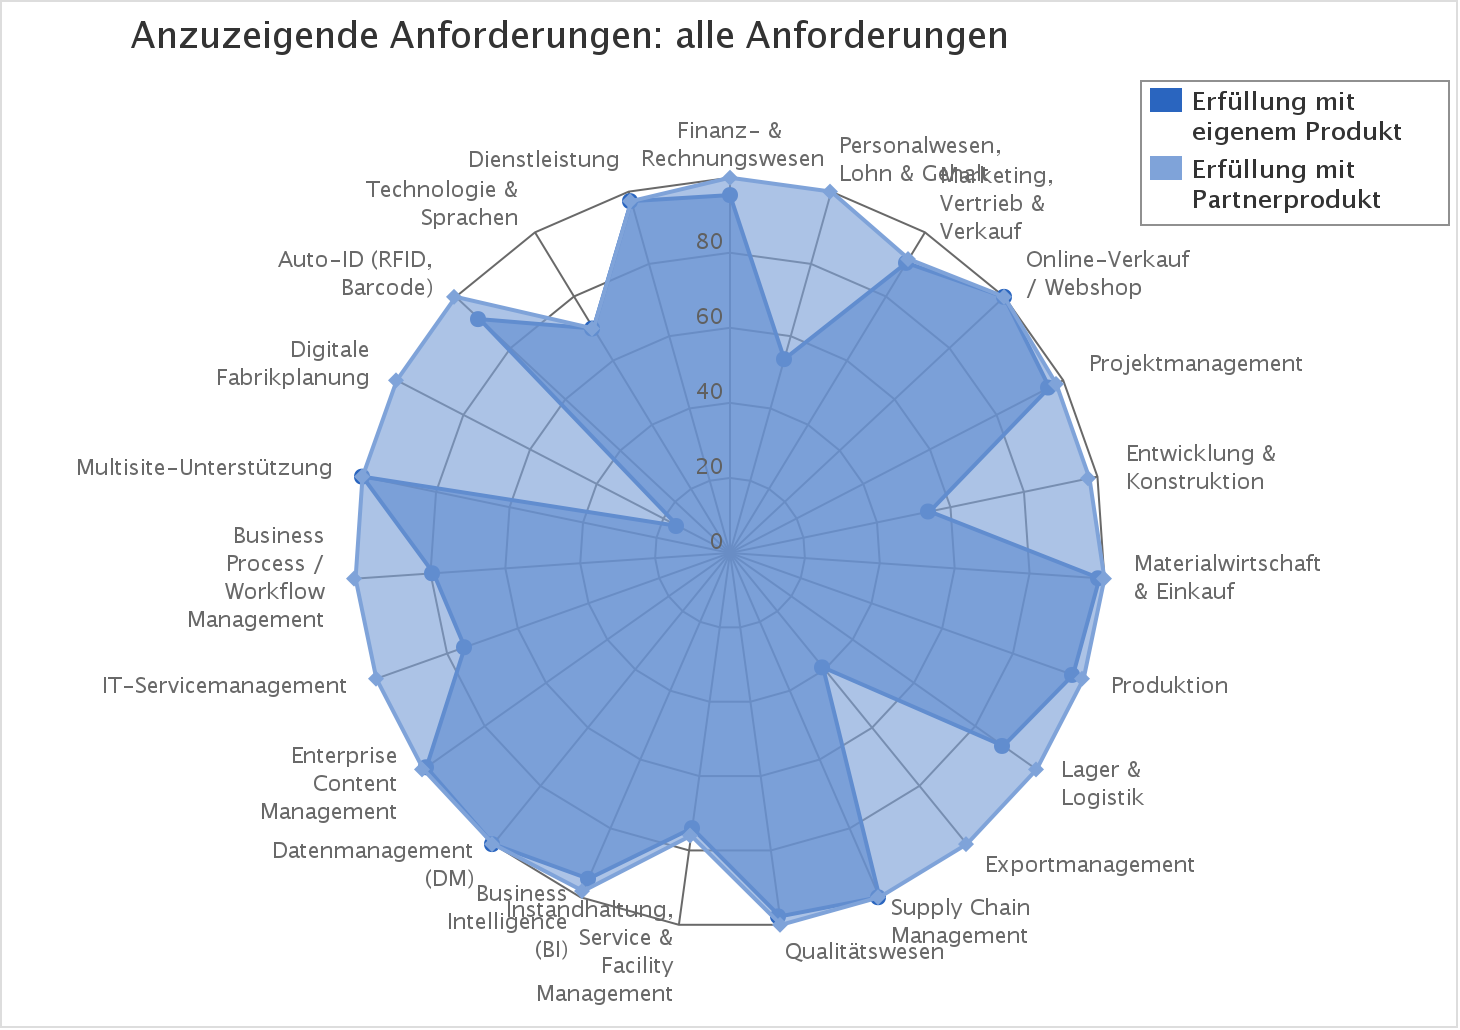
\includegraphics[width=0.7\textwidth]{images/TROVARIT_Microsoft}
\caption{Das Spinnennetz von Microsoft Dynamics NAV 2012}

\end{figure}\FloatBarrier
\noindent

\item Microsoft Dynamics NAV 2012\\
		84\% Erfüllung mit eigenem Produkt\\
		97\% Erfüllung mit Partnerprodukt\\				
		
		Nachteile: 
Vertriebsstrategien werden in diesem ERP System nicht unterstützt. Diese Sparte fällt komplett weg.
Genauso wie die Sparte des Facility Managements.
Dieses ERP System ist nicht Datenbankunabhängig und unterstützt keine Schnittstellen zu sozialen Netzwerken bezüglich Marketing.
Nicht alle Sprachen werden Unterstützt die wir uns vorgestellt hatten. Unter anderem Hindi und Slowenisch werden nicht zur Verfügung gestellt.
Zudem wird nur Windows als Betriebssystem und Server unterstützt.
 
		
\FloatBarrier
\begin{figure}[!h]
\centering
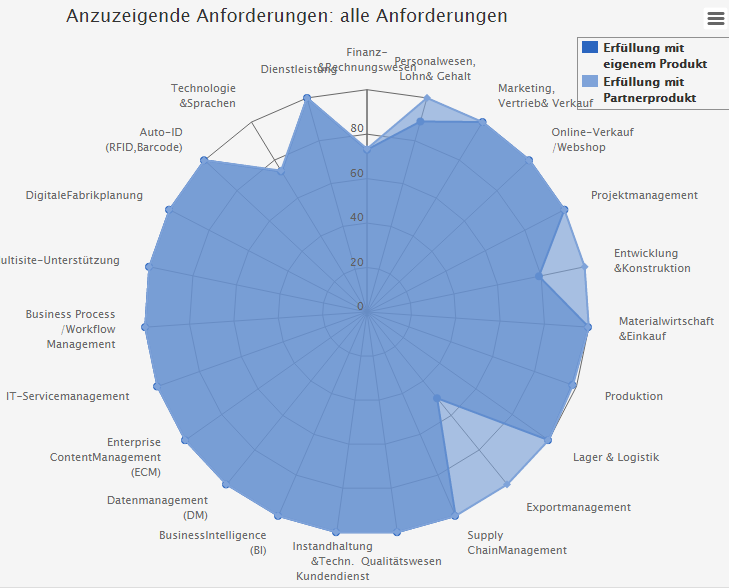
\includegraphics[width=0.7\textwidth]{images/matching4}
\caption{Die Spinnennetz von Microsoft Dynamics NAV}
\end{figure}\FloatBarrier
\noindent


\end{itemize}

\subsection{Unsere ERP-System Auswahl}
Wir haben uns für das Produkt der Itelligence AG entschieden, da sie unsere Anforderungen, ohne der Benutzung von Partnerprodukten, besser abdecken kann.  Außerdem sind die Teilbereiche, welche das System nicht abdeckt, hauptsächlich optional.
 \\ \\

%\section*{Projekthandbuch}
%\section*{Pflichtenheft}
%\section*{Vorbereitung Kick Off Meeting}

\small
\newpage\newpage
\begin{thebibliography}{56}

 \bibitem{ec1} 
  \textbf{Beetling back to success}, Jun 24th 2014, P.E, The Economist\\
  \textit{http://www.economist.com/blogs/schumpeter/2014/06/volkswagen-america}
  \newline last used: 02.02.2016
  
   
 \bibitem{ec2} 
  \textbf{VW conquers the world - Germany’s biggest carmaker is leaving rivals in the dust}\\, Jul 7th 2012 , The Economist\\
  \textit{  http://www.economist.com/node/21558269}
  \newline last used: 02.02.2016
  
    
   
 \bibitem{ec3} 
  \textbf{Europe goes electric - The Frankfurt motor show
}\\Sep 12th 2013 , P.E., The Economist\\
  \textit{  http://www.economist.com/node/21558269}
  \newline last used: 02.02.2016
  
   \bibitem{vsc50y} 
  \textbf{Volkswagen Share celebrates its 50th birthday}\\ Jun 4th 2011 , Volkswagen AG\\
  \textit{http://www.volkswagenag.com/content/vwcorp/info\_center/en/themes/2011/04/\\Volkswagen\_Share\_celebrates\_its\_50th\_birthday.html
}
  \newline last used: 02.02.2016
  
   \bibitem{2008kurs} 
  \textbf{Volkswagen Share celebrates its 50th birthday}\\ Jun 4th 2011 , Volkswagen AG\\
  \textit{  http://www.boerse.de/boersenwissen/boersengeschichte/Kurskapriolen-der-VW-Aktie-2008-\%7C45}
  \newline last used: 02.02.2016
  

   \bibitem{jbilanz2013vw} 
  \textbf{ABSCHLUSS VOLKSWAGEN AG }, 2013 \\
  \textit{ http://www.volkswagenag.com/content/vwcorp/info\_center/de/publications/2014/03/\\Financial\_Statements\_VWAG\_2013.bin.html/binarystorageitem/file/Abschluss+Volkswagen+AG+2013\_deutsch.pdf  
}
  \newline last used: 02.02.2016
    
    
       \bibitem{aktionaersstruktur} 
  \textbf{Aktionärsstruktur Volkswagen AG}, Stand 31.12.2014 \\
  \textit{http://www.volkswagenag.com/content/vwcorp/content/\\de/investor\_relations/share/Shareholder\_Structure.html}
  \newline last used: 02.02.2016
    
  \bibitem{structure1} 
  \textbf{Struktur und Geschäftstätigkeit}\\
  \textit{http://www.volkswagenag.com/content/gb2007/content/de/corporate\_governance/\\structure\_and\_business\_activities\_\_part\_of\_the\_management\_report\_.html}
  \newline last used: 02.02.2016
  
  \bibitem{domavw} 
  \textbf{Aufbauorganisation der Volkswagen AG}, volkswagenag.com \\
  \textit{http://bauhaus.cs.uni-magdeburg.de:8080/miscms.nsf/FEA8C8150500AA14C1257449004F79A9\\/CE79949E8E27681DC12579C1006D9A27/\$FILE/Diplomarbeit\%20Oliver\%20Meier.pdf}
  \newline last used: 02.02.2016  
  
       \bibitem{2008wtf} 
 \textbf{Short sellers make VW the world's priciest firm}, reuters.com. SARAH Marsh \\
  \textit{  http://www.reuters.com/article/2008/10/28/us-volkswagen-idUSTRE49R3I920081028}
  \newline last used: 02.02.2016 
  
         \bibitem{aktienfotos} 
 \textbf{Vorzugs- und Stammaktien}, volkswagenag.com \\
  \textit{   http://www.volkswagenag.com/content/vwcorp/content/de/investor\_relations/share.html}
  \newline last used: 02.02.2016
  
  \bibitem{marken} 
 \textbf{Web Ressource}, marketbusinessnews.com \\
  \textit{   http://marketbusinessnews.com/wp-content/uploads/2014/02/Volkswagen-Group-Brands.png}
  \newline last used: 02.02.2016
  
  \bibitem{produktionsstandorte} 
 \textbf{Produktionsstandorte}, mvolkswagenag.com \\
  \textit{   http://www.volkswagenag.com/content/vwcorp/content/de/the\_group/production\_plants.html}
  \newline last used: 02.02.2016
  
  \bibitem{struktur} 
 \textbf{Struktur und Geschäftstätigkeit}, volkswagenag.com \\
  \textit{	http://www.volkswagenag.com/content/gb2007/content/de/corporate\_governance\\/structure\_and\_business\_activities\_\_part\_of\_the\_management\_report\_.html}
  \newline last used: 02.02.2016  

      \bibitem{yahoofinanzenvw} 
 \textbf{Volkswagen AG},Yahoo Finanzen \\
  \textit{  https://de.finance.yahoo.com/q/ks?s=VOW3.DE}
  \newline last used: 02.02.2016 
  
        \bibitem{vwwebsitestrat} 
 \textbf{Volkswagen AG Strategie},volkswagenag.com \\
  \textit{http://www.volkswagenag.com/content/vwcorp/content/de/the\_group/strategy.html}
  \newline last used: 02.02.2016  
    
      \bibitem{vwwebsitechina} 
 \textbf{Markt Spezial: China},volkswagenag.com \\
  \textit{http://www.volkswagenag.com/content/vwcorp/content/de/investor\\\_relations/Warum\_Volkswagen/Marke\_Focus.html
}
  \newline last used: 02.02.2016
  \bibitem{geschdautos} 
  \textbf{Geschichte des Autos} \\
  \textit{
  	http://www.fundus.org/referat.asp?ID=11034
  }
  \newline last used: 02.02.2016
  
  
  \bibitem{autowp} 
  \textbf{Entstehungsgeschichte von VW} \\
  \textit{
  	http://www.autowallpaper.de/Wallpaper/VW/Entstehungsgeschichte\_VW.htm
  }
  \newline last used: 02.02.2016
  
  \bibitem{terror} 
  \textbf{Wolfgang Benz, Barbara Distel}, 2005-2009 \\
  \textit{
  	Der Ort des Terrors. Geschichte der nationalsozialistischen Konzentrationslager
  }
  
  
  \bibitem{ahwest} 
  \textbf{Volgswagen AG Geschichte} \\
  \textit{
  	http://www.autohaus-westend.de/volkswagen-ag-geschichte/
  }
  \newline last used: 02.02.2016
  
  \bibitem{vwag} 
  \textbf{Volgswagen AG} \\
  \textit{
  	http://www.volkswagenag.com/
  }
  \newline last used: 02.02.2016
  
  \bibitem{sud} 
  \textbf{Drastische Gewinneinbruch bei VW} \\
  \textit{
  	http://www.sueddeutsche.de/wirtschaft/geschaeftsjahr-drastischer-gewinneinbruch-bei-vw-1.814556
  }
  \newline last used: 02.02.2016
  
  \bibitem{vwchronik} 
  \textbf{VW Chronik} \\
  \textit{
  	http://www.chronik.volkswagenag.com/
  }
  \newline last used: 02.02.2016

\bibitem{fspic} 
\textbf{Francisco Sanz Bild} \\
\textit{
	http://autogramm.volkswagen.de/07-08\_12/images/content/popups/23\_Sanz.jpg
}
\newline last used: 02.02.2016

\bibitem{jhpic} 
\textbf{Jochem Heizmann Bild} \\
\textit{
	http://autogramm.volkswagen.de/08\_10/images/content/popups/07\_P\_heizmann.jpg
}
\newline last used: 02.02.2016

\bibitem{ckpic} 
\textbf{Christian Klingler Bild} \\
\textit{
	http://www.produktion.de/wp-content/uploads/2014/04/christian\_klingler.jpg
}
\newline last used: 02.02.2016

\bibitem{mmpic} 
\textbf{Matthias Mueller Bild} \\
\textit{
	http://fotos.autozeitung.de/938x704/images/bildergalerie/2015/02/porsche-matthias-mueller.jpg
}
\newline last used: 02.02.2016

\bibitem{hnpic} 
\textbf{Horst Neumann Bild} \\
\textit{
	http://www.astroman.com.pl/img/magazyn/1376/o/Horst\_Neumann\_1.jpg
}
\newline last used: 02.02.2016

\bibitem{arpic} 
\textbf{Andreas Renschler Bild} \\
\textit{
	http://transportnet.se/files/2014/02/AndreasRenschler.jpg
}
\newline last used: 02.02.2016

\bibitem{hppic} 
\textbf{Hans Poetsch Bild} \\
\textit{
	http://www.automobil-produktion.de/uploads/2011/03/vw\_poetsch-229x300.jpg
}
\newline last used: 02.02.2016

\bibitem{rspic} 
\textbf{Rupert Stadler Bild} \\
\textit{
	http://www.matthiashaslauer.com/corporate/stadler/haslauer\_1.jpg
}
\newline last used: 02.02.2016

\bibitem{vwlogistics} 
\textbf{Volkswagen Logistics} \\
\textit{
	http://www.volkswagen-logistics.com/
}
\newline last used: 02.02.2016

\bibitem{vwlogisticspic} 
\textbf{Volkswagen Logistics Bild} \\
\textit{
	http://gvz-e-wolfsburg.de/images/logologistics.jpg
}
\newline last used: 02.02.2016

\bibitem{vorstand} 
\textbf{Volkswagen AG Vorstand} \\
\textit{
	http://www.volkswagenag.com/content/vwcorp/content/de/the\_group/senior\_management.html
}
\newline last used: 02.02.2016

\bibitem{wolfsburg} 
\textbf{Wolfsburg Fachtagung} \\
\textit{
	http://autogramm.volkswagen.de/09\_13/wolfsburg/wolfsburg\_01.html
}
\newline last used: 02.02.2016

\bibitem{poetschbio} 
\textbf{Poetsch Biographie} \\
\textit{
	http://www.volkswagenag.com/content/vwcorp/content/de/the\_group/senior\_management/poetsch.html
}
\newline last used: 02.02.2016

\bibitem{vw-produkte} 
\textbf{Volkswagen Navigator} \\
\textit{
	http://navigator.volkswagenag.com/index.html
}
\newline last used: 02.02.2016


\bibitem{vwamstrategie} 
\textbf{Neue Volkswagen-Strategie: Winterkorns Wende},Michael Kröger \\
\textit{http://www.spiegel.de/wirtschaft/unternehmen/vw-jahresbilanz-volkswagen-chef-winterkorn-mit-neuer-strategie-a-958439.html}
\newline last used: 02.02.2016


\bibitem{vwamstrategiechina} 
\textbf{Volkswagen will mit länderspezifischen Strategien an die Weltspitze}, dw.de \\
\textit{http://www.dw.de/volkswagen-will-mit-l\%C3\%A4\\nderspezifischen-strategien-an-die-weltspitze/a-17356433}
\newline last used: 02.02.2016



\bibitem{vwamstrategiechina2} 
\textbf{VW drückt in China mächtig aufs Tempo}, Wirtschafts Woche \\
\textit{http://www.wiwo.de/unternehmen/auto/werke-sollen-schnell-eroeffnen-vw-entspricht-chinas-go-west-strategie/8488212-2.html}
\newline last used: 02.02.2016

\bibitem{vwamstrategie3} 
\textbf{Jahrespressekonferenz 2012}, Volkswagen AG \\
\textit{http://www.volkswagenag.com/content/vwcorp/info\_center/de/talks\_and\_presentations/2012/03/JPK\_IK\_2012\_Part\_III.bin.html/binarystorageitem/file/Teil\_III\_Charts\_Winterkorn.pdf}
\newline last used: 02.02.2016

\bibitem{mqb} 
\textbf{Volkswagen MQB} \\
\textit{
	http://www.volkswagenag.com/content/vwcorp/content/de/investor\_relations/Warum\_Volkswagen/MQB.html
}
\newline last used: 02.02.2016

\bibitem{baukastengraph} 
\textbf{Volkswagen Baukästen} \\
\textit{
	http://www.volkswagenag.com/content/vwcorp/content/de/investor\\ \_relations/Warum\_Volkswagen/MQB.img.html/contentparsys/textandimages/images/textbinary/image/MQB1.png
}
\newline last used: 02.02.2016

\bibitem{mqbdefault} 
\textbf{Volkswagen MQB} \\
\textit{
	http://www.volkswagenag.com/content/vwcorp/content/de/investor\\ \_relations/Warum\_Volkswagen/MQB.img.html/contentparsys/textandimages/images/textbinary\_0/image/MQB2.png
}
\newline last used: 02.02.2016

\bibitem{squeezy} 
\textbf{Squeezy money - Porsche and VW} economist.com \\
\textit{http://www.economist.com/node/12523898}
\newline last used: 02.02.2016

\bibitem{audiRinge} 
\textbf{Vier Marken - Vier Ringe} audi.com \\
\textit{http://www.audi.com/corporate/de/unternehmen/historie/unternehmen-und-marken/vier-marken-vier-ringe.html}
\newline last used: 02.02.2016

\bibitem{audiNeuwagen} 
\textbf{Audi - Neuwagen} audi.de \\
\textit{http://www.audi.de/de/brand/de/neuwagen.html}
\newline last used: 02.02.2016

\bibitem{vwPorscheUebernahme} 
\textbf{Die Presse - Volkswagen schließt Porsche-Übernahme ab} diepresse.com \\
\textit{http://diepresse.com/home/wirtschaft/international/1274167/Volkswagen-schliesst-PorscheUebernahme-ab}
\newline last used: 02.02.2016

\bibitem{ScaniaMAN} 
\textbf{VW/Scania – "Der Deal macht keinen Sinn"} wirtschaftsblatt.at \\
\textit{http://wirtschaftsblatt.at/home/boerse/europa/1566768/VWScania-Der-Deal-macht-keinen-Sinn}
\newline last used: 02.02.2016

\bibitem{adsfhgterwdsfhgf} 
\textbf{Porsche Holding Bericht} \\
\textit{http://www.bafin.de/SharedDocs/Downloads/DE/Befreiungsentscheidung/volkswagen\\\_ag\_ua.pdf?\_\_blob=publicationFile\&v=5
}
\newline last used: 02.02.2016


\bibitem{adsfhgterwdsfhgf2} 
\textbf{Vorzugsaktien - Neue Blüte dank VW}, Frankfurter Allgemeine \\
\textit{http://www.faz.net/aktuell/finanzen/aktien/vorzugsaktien-neue-bluete-dank-vw-1894737/infografik-volkswagen-henkel-1903555.html}
\newline last used: 02.02.2016



\end{thebibliography}
\end{document}
%img : httpmarkets.ft.comresearchMarketsTearsheetsSummarys=VOWBER vwdax.PNG
% http://www.statista.com/statistics/257660/passenger-car-sales-in-selected-countries/ salesla
% http://www.statista.com/statistics/232958/revenue-of-the-leading-car-manufacturers-worldwide/ revenu
